\documentclass[10pt,fleqn]{article} % Default font size and left-justified equations
\usepackage[%
    pdftitle={SLCI : Cinématique du solide},
    pdfauthor={Xavier Pessoles}]{hyperref}

%%%%%%%%%%%%%%%%%%%%%%%%%%%%%%%%%%%%%%%%%
% Original author:
% Mathias Legrand (legrand.mathias@gmail.com) with modifications by:
% Vel (vel@latextemplates.com)
% License:
% CC BY-NC-SA 3.0 (http://creativecommons.org/licenses/by-nc-sa/3.0/)
%%%%%%%%%%%%%%%%%%%%%%%%%%%%%%%%%%%%%%%%%

%----------------------------------------------------------------------------------------
%	VARIOUS REQUIRED PACKAGES AND CONFIGURATIONS
%----------------------------------------------------------------------------------------

\usepackage[top=2.5cm,bottom=2cm,left=2cm,right=2cm,headsep=40pt,a4paper]{geometry} % Page margins

\usepackage{graphicx} % Required for including pictures
\graphicspath{{images/}} % Specifies the directory where pictures are stored

\usepackage{lipsum} % Inserts dummy text

\usepackage{tikz} % Required for drawing custom shapes

\usepackage[french]{babel} % English language/hyphenation
\frenchbsetup{StandardLists=true} % Pour éviter la collision babel enumitem pour les listes

\usepackage{enumitem} % Customize lists
\setlist{nolistsep} % Reduce spacing between bullet points and numbered lists

\usepackage{booktabs} % Required for nicer horizontal rules in tables

\usepackage{xcolor} % Required for specifying colors by name
%\definecolor{ocre}{RGB}{243,102,25} % Define the orange color used for highlighting throughout the book
 \definecolor{ocre}{RGB}{49,133,156} % Couleur ''bleue''
\definecolor{violetf}{RGB}{112,48,160} % Couleur ''violet''
\usepackage{enumitem}
\usepackage{pifont} % Pour les dinglist
\usepackage{multicol}
\usepackage{array} % Centrage vertical dans les tableaux

%----------------------------------------------------------------------------------------
%	FONTS
%----------------------------------------------------------------------------------------

\usepackage{avant} % Use the Avantgarde font for headings
%\usepackage{times} % Use the Times font for headings
%\usepackage{mathptmx} % Use the Adobe Times Roman as the default text font together with math symbols from the Sym­bol, Chancery and Com­puter Modern fonts
\usepackage[adobe-utopia]{mathdesign}
\usepackage{microtype} % Slightly tweak font spacing for aesthetics
\usepackage[utf8]{inputenc} % Required for including letters with accents
\usepackage[T1]{fontenc} % Use 8-bit encoding that has 256 glyphs

%----------------------------------------------------------------------------------------
%	BIBLIOGRAPHY AND INDEX
%----------------------------------------------------------------------------------------

\usepackage[style=alphabetic,citestyle=numeric,sorting=nyt,sortcites=true,autopunct=true,babel=hyphen,hyperref=true,abbreviate=false,backref=true,backend=biber]{biblatex}
\addbibresource{bibliography.bib} % BibTeX bibliography file
\defbibheading{bibempty}{}

\usepackage{calc} % For simpler calculation - used for spacing the index letter headings correctly
\usepackage{makeidx} % Required to make an index
\makeindex % Tells LaTeX to create the files required for indexing

%----------------------------------------------------------------------------------------
%	MAIN TABLE OF CONTENTS
%----------------------------------------------------------------------------------------

\usepackage{titletoc} % Required for manipulating the table of contents

\setcounter{tocdepth}{2}     % Dans la table des matieres
\setcounter{secnumdepth}{2}

\contentsmargin{0cm} % Removes the default margin

% Part text styling
\titlecontents{part}[0cm]
{\addvspace{20pt}\centering\large\bfseries}
{}
{}
{}

% Chapter text styling
\titlecontents{chapter}[1.25cm] % Indentation
{\addvspace{12pt}\large\sffamily\bfseries} % Spacing and font options for chapters
{\color{ocre!60}\contentslabel[\Large\thecontentslabel]{1.25cm}\color{ocre}} % Chapter number
{\color{ocre}}  
{\color{ocre!60}\normalsize\;\titlerule*[.5pc]{.}\;\thecontentspage} % Page number

% Section text styling
\titlecontents{section}[1.25cm] % Indentation
{\addvspace{3pt}\sffamily\bfseries} % Spacing and font options for sections
{\color{ocre!60}\contentslabel[\thecontentslabel]{1.25cm} \color{ocre}} % Section number
{\color{ocre}}
{\hfill\color{ocre!60}\thecontentspage} % Page number
[]

% Subsection text styling
\titlecontents{subsection}[1.25cm] % Indentation
{\addvspace{1pt}\sffamily\small} % Spacing and font options for subsections
{\contentslabel[\thecontentslabel]{1.25cm}} % Subsection number
{}
{\ \titlerule*[.5pc]{.}\;\thecontentspage} % Page number
[]


% Subsection text styling
\titlecontents{subsubsection}[1.25cm] % Indentation
{\addvspace{1pt}\sffamily\small} % Spacing and font options for subsections
{\contentslabel[\thecontentslabel]{1.25cm}} % Subsection number
{}
{\ \titlerule*[.5pc]{.}\;\thecontentspage} % Page number
[]

% List of figures
\titlecontents{figure}[0em]
{\addvspace{-5pt}\sffamily}
{\thecontentslabel\hspace*{1em}}
{}
{\ \titlerule*[.5pc]{.}\;\thecontentspage}
[]

% List of tables
\titlecontents{table}[0em]
{\addvspace{-5pt}\sffamily}
{\thecontentslabel\hspace*{1em}}
{}
{\ \titlerule*[.5pc]{.}\;\thecontentspage}
[]

%----------------------------------------------------------------------------------------
%	MINI TABLE OF CONTENTS IN PART HEADS
%----------------------------------------------------------------------------------------

% Chapter text styling
\titlecontents{lchapter}[0em] % Indenting
{\addvspace{15pt}\large\sffamily\bfseries} % Spacing and font options for chapters
{\color{ocre}\contentslabel[\Large\thecontentslabel]{1.25cm}\color{ocre}} % Chapter number
{}  
{\color{ocre}\normalsize\sffamily\bfseries\;\titlerule*[.5pc]{.}\;\thecontentspage} % Page number

% Section text styling
\titlecontents{lsection}[0em] % Indenting
{\sffamily\small} % Spacing and font options for sections
{\contentslabel[\thecontentslabel]{1.25cm}} % Section number
{}
{}

% Subsection text styling
\titlecontents{lsubsection}[.5em] % Indentation
{\normalfont\footnotesize\sffamily} % Font settings
{}
{}
{}

%----------------------------------------------------------------------------------------
%	PAGE HEADERS
%----------------------------------------------------------------------------------------

\usepackage{fancyhdr} % Required for header and footer configuration



\pagestyle{fancy}
 \renewcommand{\headrulewidth}{0pt}
 \fancyhead{}
 \fancyhead[L]{%
 \noindent\begin{minipage}[c]{2.6cm}%
 
\includegraphics[width=2cm]{png/logo_lycee.png}%
 \end{minipage}}

\fancyhead[C]{\rule{8cm}{.5pt}}

 \fancyhead[R]{%
 \noindent\begin{minipage}[c]{3cm}
 \begin{flushright}
 \footnotesize{\textit{\textsf{\xxtete}}}%
 \end{flushright}
 \end{minipage}
}


\fancyfoot[C]{\rule{12cm}{.5pt}}
\renewcommand{\footrulewidth}{0.2pt}
\fancyfoot[C]{\footnotesize{\bfseries \thepage}}
\fancyfoot[L]{ 
\begin{minipage}[c]{.4\linewidth}
\noindent\footnotesize{{\xxauteur}}
\end{minipage}}


\fancyfoot[R]{\footnotesize{\xxpied}
\ifthenelse{\isodd{\value{page}}}{
\begin{tikzpicture}[overlay]
\node[shape=rectangle, 
      rounded corners = .25 cm,
	  draw= ocre,
	  line width=2pt, 
	  fill = ocre!10,
	  minimum width  = 2.5cm,
	  minimum height = 3cm,] at (\xxposongletx,\xxposonglety) {};
\node at (\xxposonglettext,\xxposonglety) {\rotatebox{90}{\textbf{\large\color{ocre}{\xxonglet}}}};
%{};
\end{tikzpicture}}{}
}
%
%
%
% Removes the header from odd empty pages at the end of chapters
\makeatletter
\renewcommand{\cleardoublepage}{
\clearpage\ifodd\c@page\else
\hbox{}
\vspace*{\fill}
\thispagestyle{empty}
\newpage
\fi}

\fancypagestyle{plain}{%
\fancyhf{} % vide l’en-tête et le pied~de~page.
%\fancyfoot[C]{\bfseries \thepage} % numéro de la page en cours en gras
% et centré en pied~de~page.
\fancyfoot[R]{\footnotesize{\xxpied}}
\fancyfoot[C]{\rule{12cm}{.5pt}}
\renewcommand{\footrulewidth}{0.2pt}
\fancyfoot[C]{\footnotesize{\bfseries \thepage}}
\fancyfoot[L]{ 
\begin{minipage}[c]{.4\linewidth}
\noindent\footnotesize{{\xxauteur}}
\end{minipage}}}



%----------------------------------------------------------------------------------------
%	THEOREM STYLES
%----------------------------------------------------------------------------------------

% Conflit avec la police adobe
%\usepackage{amsmath,amsfonts,amssymb,amsthm} % For math equations, theorems, symbols, etc
\usepackage{amsmath,amsthm}

\newcommand{\intoo}[2]{\mathopen{]}#1\,;#2\mathclose{[}}
\newcommand{\ud}{\mathop{\mathrm{{}d}}\mathopen{}}
\newcommand{\intff}[2]{\mathopen{[}#1\,;#2\mathclose{]}}
%\newtheorem{notation}{Notation}[chapter]
\newtheorem{notation}{Notation}[section]

% Boxed/framed environments
\newtheoremstyle{ocrenumbox}% % Theorem style name
{0pt}% Space above
{0pt}% Space below
{\normalfont}% % Body font
{}% Indent amount
{\small\bf\sffamily\color{ocre}}% % Theorem head font
{\;}% Punctuation after theorem head
{0.25em}% Space after theorem head
{\small\sffamily\color{ocre}\thmname{#1}\nobreakspace\thmnumber%{\@ifnotempty{#1}{}\@upn{#2}}% Theorem text (e.g. Theorem 2.1)
\thmnote{\nobreakspace\the\thm@notefont\sffamily\bfseries\color{black}---\nobreakspace#3.}} % Optional theorem note
\renewcommand{\qedsymbol}{$\blacksquare$}% Optional qed square


% Boite pour les corriges
\newtheoremstyle{correctionbox}% % Theorem style name
{0pt}% Space above
{0pt}% Space below
{\normalfont}% % Body font
{}% Indent amount
{\small\bf\sffamily\color{violet}}% % Theorem head font
{\;}% Punctuation after theorem head
{0.25em}% Space after theorem head
{\small\sffamily\color{ocre}\thmname{#1}\nobreakspace\thmnumber%{\@ifnotempty{#1}{}\@upn{#2}}% Theorem text (e.g. Theorem 2.1)
\thmnote{\nobreakspace\the\thm@notefont\sffamily\bfseries\color{black}---\nobreakspace#3.}} % Optional theorem note
\renewcommand{\qedsymbol}{$\blacksquare$}% Optional qed square



\newtheoremstyle{blacknumex}% Theorem style name
{5pt}% Space above
{5pt}% Space below
{\normalfont}% Body font
{} % Indent amount
{\small\bf\sffamily}% Theorem head font
{\;}% Punctuation after theorem head
{0.25em}% Space after theorem head
{\small\sffamily{\tiny\ensuremath{\blacksquare}}\nobreakspace\thmname{#1}\nobreakspace\thmnumber%{\@ifnotempty{#1}{}\@upn{#2}}% Theorem text (e.g. Theorem 2.1)
\thmnote{\nobreakspace\the\thm@notefont\sffamily\bfseries---\nobreakspace#3.}}% Optional theorem note

\newtheoremstyle{blacknumbox} % Theorem style name
{0pt}% Space above
{0pt}% Space below
{\normalfont}% Body font
{}% Indent amount
{\small\bf\sffamily}% Theorem head font
{\;}% Punctuation after theorem head
{0.25em}% Space after theorem head
{\small\sffamily\thmname{#1}\nobreakspace 
\thmnote{\nobreakspace\the\thm@notefont\sffamily\bfseries---\nobreakspace#3.}}% Optional theorem note

% Non-boxed/non-framed environments
\newtheoremstyle{ocrenum}% % Theorem style name
{5pt}% Space above
{5pt}% Space below
{\normalfont}% % Body font
{}% Indent amount
{\small\bf\sffamily\color{ocre}}% % Theorem head font
{\;}% Punctuation after theorem head
{0.25em}% Space after theorem head
{\small\sffamily\color{ocre}\thmname{#1}\nobreakspace%\thmnumber{\@ifnotempty{#1}{}\@upn{#2}}% Theorem text (e.g. Theorem 2.1)
\thmnote{\nobreakspace\the\thm@notefont\sffamily\bfseries\color{black}---\nobreakspace#3.}} % Optional theorem note
\renewcommand{\qedsymbol}{$\blacksquare$}% Optional qed square
\makeatother

% Environnement pour les titres de parties
\newtheoremstyle{partiebox} 
{0pt}% Space above
{0pt}% Space below
{\normalfont}% Body font
{}% Indent amount
{\small\bf\sffamily}% Theorem head font
{\;}% Punctuation after theorem head
{0.25em}% Space after theorem head




% Defines the theorem text style for each type of theorem to one of the three styles above
\newcounter{dummy} 
\numberwithin{dummy}{section}
\theoremstyle{ocrenumbox}
%\newtheorem{theoremeT}[dummy]{Théorème}
\newtheorem{theoremeT}[dummy]{Théorème}
\newtheorem{resultatT}[dummy]{Résultat}
\newtheorem{savoirT}[dummy]{Savoir}
\newtheorem{methodeT}[dummy]{Méthode}
\newtheorem{objectifT}[dummy]{Objectif}
%\newtheorem{problem}{Problem}[chapter]
\newtheorem{problem}{Problem}[section]
%\newtheorem{exerciseT}{Exercise}[chapter]
\newtheorem{exerciseT}{Exercice}[section]

\theoremstyle{blacknumex}
%\newtheorem{exampleT}{Example}[chapter]
\newtheorem{exempleT}{Exemple}[section]
\newtheorem{termT}{Terminal\\}[section]
\newtheorem{pyT}{Python\\}[section]
\newtheorem{sciT}{Scilab\\}[section]
\newtheorem{pseudoT}{Pseudo Code\\}[section]
\newtheorem{sqlT}{SQL\\}[section]

\theoremstyle{blacknumbox}
%\newtheorem{vocabulary}{Vocabulary}[chapter]
\newtheorem{vocabulary}{Vocabulaire}[section]
%\newtheorem{definitionT}{Definition}[section]
\newtheorem{definitionT}{Définition}[section]
\newtheorem{rappelT}{Rappel}[section]
\newtheorem{demoT}{Démonstration}[section]
\newtheorem{corollaryT}[dummy]{Corollaire}
\newtheorem{hypoT}{Hypothèse(s)}

\theoremstyle{ocrenum}
\newtheorem{proposition}[dummy]{Proposition}

\theoremstyle{partiebox}
\newtheorem{titrepartieT}[]{}
\newtheorem{titrechapitreT}[]{}

\theoremstyle{correctionbox}
\newtheorem{correctionT}[dummy]{\color{violet}{Correction}}

%----------------------------------------------------------------------------------------
%	DEFINITION OF COLORED BOXES
%----------------------------------------------------------------------------------------

\RequirePackage[framemethod=tikz]{mdframed} % Required for creating the theorem, definition, exercise and corollary boxes

% Theorem box
\newmdenv[skipabove=7pt,
skipbelow=7pt,
backgroundcolor=ocre!10,
linecolor=ocre,
innerleftmargin=5pt,
innerrightmargin=5pt,
innertopmargin=5pt,
leftmargin=0cm,
rightmargin=0cm,
innerbottommargin=5pt]{tBox}


% Correction
\newmdenv[skipabove=7pt,
skipbelow=7pt,
backgroundcolor=violet!10,
linecolor=violet,
innerleftmargin=5pt,
innerrightmargin=5pt,
innertopmargin=5pt,
leftmargin=0cm,
rightmargin=0cm,
innerbottommargin=5pt]{coBox}


% Exercise box	  
\newmdenv[skipabove=7pt,
skipbelow=7pt,
rightline=false,
leftline=true,
topline=false,
bottomline=false,
backgroundcolor=ocre!10,
linecolor=ocre,
innerleftmargin=5pt,
innerrightmargin=5pt,
innertopmargin=5pt,
innerbottommargin=5pt,
leftmargin=0cm,
rightmargin=0cm,
linewidth=4pt]{eBox}	

% Definition box
\newmdenv[skipabove=7pt,
skipbelow=7pt,
rightline=false,
leftline=true,
topline=false,
bottomline=false,
backgroundcolor=ocre!10,
linecolor=ocre,
innerleftmargin=5pt,
innerrightmargin=5pt,
innertopmargin=0pt,
leftmargin=0cm,
rightmargin=0cm,
linewidth=4pt,
innerbottommargin=0pt]{dBox}	

% Demonstration box
\newmdenv[skipabove=7pt,
skipbelow=7pt,
rightline=false,
leftline=true,
topline=false,
bottomline=false,
%backgroundcolor=ocre!10,
linecolor=ocre,
innerleftmargin=5pt,
innerrightmargin=5pt,
innertopmargin=0pt,
leftmargin=0cm,
rightmargin=0cm,
linewidth=4pt,
innerbottommargin=0pt]{demoBox}	

% Corollary box
\newmdenv[skipabove=7pt,
skipbelow=7pt,
rightline=false,
leftline=true,
topline=false,
bottomline=false,
linecolor=gray,
backgroundcolor=black!5,
innerleftmargin=5pt,
innerrightmargin=5pt,
innertopmargin=5pt,
leftmargin=0cm,
rightmargin=0cm,
linewidth=4pt,
innerbottommargin=5pt]{cBox}


% Hypothèses
\newmdenv[skipabove=7pt,
skipbelow=7pt,
rightline=false,
leftline=true,
topline=false,
bottomline=false,
linecolor=gray,
backgroundcolor=black!5,
innerleftmargin=5pt,
innerrightmargin=5pt,
innertopmargin=5pt,
leftmargin=0cm,
rightmargin=0cm,
linewidth=4pt,
innerbottommargin=5pt]{hyBox}


% Boite pour le titre de la partie (pBox)
\newmdenv[skipabove=7pt,
skipbelow=7pt,
rightline=true,
leftline=false,
topline=false,
bottomline=false,
linecolor=ocre,
backgroundcolor=none,
innerleftmargin=5pt,
innerrightmargin=5pt,
innertopmargin=5pt,
leftmargin=0cm,
rightmargin=0cm,
linewidth=4pt,
innerbottommargin=5pt]{pBox}

% Boite pour le titre du chapitre (chBox)
\newmdenv[skipabove=7pt,
skipbelow=7pt,
rightline=false,
leftline=true,
topline=false,
bottomline=false,
linecolor=ocre,
%backgroundcolor=black!5,
innerleftmargin=5pt,
innerrightmargin=5pt,
innertopmargin=5pt,
leftmargin=0cm,
rightmargin=0cm,
linewidth=4pt,
innerbottommargin=5pt]{chBox}


% Boite pour les exemples
\newmdenv[skipabove=7pt,
skipbelow=7pt,
rightline=false,
leftline=true,
topline=false,
bottomline=false,
linecolor=gray,
backgroundcolor=white,
innerleftmargin=5pt,
innerrightmargin=5pt,
innertopmargin=5pt,
leftmargin=0cm,
rightmargin=0cm,
linewidth=4pt,
innerbottommargin=5pt]{exBox}

% Boite pour le terminal
\newmdenv[skipabove=7pt,
skipbelow=7pt,
rightline=false,
leftline=true,
topline=false,
bottomline=false,
linecolor=gray,
backgroundcolor=white,
innerleftmargin=5pt,
innerrightmargin=5pt,
innertopmargin=5pt,
leftmargin=0cm,
rightmargin=0cm,
linewidth=4pt,
innerbottommargin=5pt]{termBox}


% Boite pour Python
\newmdenv[skipabove=7pt,
skipbelow=7pt,
rightline=false,
leftline=true,
topline=false,
bottomline=false,
linecolor=gray,
backgroundcolor=white,
innerleftmargin=5pt,
innerrightmargin=5pt,
innertopmargin=0pt,
leftmargin=0cm,
rightmargin=0cm,
linewidth=4pt,
innerbottommargin=5pt]{pyBox}

% Boite pour scilab
\newmdenv[skipabove=7pt,
skipbelow=7pt,
rightline=false,
leftline=true,
topline=false,
bottomline=false,
linecolor=gray,
backgroundcolor=white,
innerleftmargin=5pt,
innerrightmargin=5pt,
innertopmargin=5pt,
leftmargin=0cm,
rightmargin=0cm,
linewidth=4pt,
innerbottommargin=5pt]{sciBox}


% Boite pour pseudo
\newmdenv[skipabove=7pt,
skipbelow=7pt,
rightline=false,
leftline=true,
topline=false,
bottomline=false,
linecolor=gray,
backgroundcolor=white,
innerleftmargin=5pt,
innerrightmargin=5pt,
innertopmargin=5pt,
leftmargin=0cm,
rightmargin=0cm,
linewidth=4pt,
innerbottommargin=5pt]{pseudoBox}

% Boite pour pseudo
\newmdenv[skipabove=7pt,
skipbelow=7pt,
rightline=false,
leftline=true,
topline=false,
bottomline=false,
linecolor=gray,
backgroundcolor=white,
innerleftmargin=5pt,
innerrightmargin=5pt,
innertopmargin=5pt,
leftmargin=0cm,
rightmargin=0cm,
linewidth=4pt,
innerbottommargin=5pt]{sqlBox}


% Creates an environment for each type of theorem and assigns it a theorem text style from the "Theorem Styles" section above and a colored box from above
\newenvironment{theorem}{\begin{tBox}\begin{theoremeT}}{\end{theoremeT}\end{tBox}}
\newenvironment{resultat}{\begin{tBox}\begin{resultatT}}{\end{resultatT}\end{tBox}}
\newenvironment{methode}{\begin{tBox}\begin{methodeT}}{\end{methodeT}\end{tBox}}
\newenvironment{savoir}{\begin{tBox}\begin{savoirT}}{\end{savoirT}\end{tBox}}
\newenvironment{obj}{\begin{tBox}\begin{objectifT}}{\end{objectifT}\end{tBox}}
\newenvironment{corrige}{\begin{coBox}\begin{correctionT}}{\end{correctionT}\end{coBox}}
\newenvironment{exercise}{\begin{eBox}\begin{exerciseT}}{\hfill{\color{ocre}\tiny\ensuremath{\blacksquare}}\end{exerciseT}\end{eBox}}				  
\newenvironment{exercice}{\begin{eBox}\begin{exerciseT}}{\hfill{\color{ocre}\tiny\ensuremath{\blacksquare}}\end{exerciseT}\end{eBox}}				  

\newenvironment{definition}{\begin{dBox}\begin{definitionT}}{\end{definitionT}\end{dBox}}	
\newenvironment{rappel}{\begin{dBox}\begin{rappelT}}{\end{rappelT}\end{dBox}}	
\newenvironment{defi}{\begin{dBox}\begin{definitionT}}{\end{definitionT}\end{dBox}}	
\newenvironment{demo}{\begin{demoBox}\begin{demoT}}{\end{demoT}\end{demoBox}}	
%\newenvironment{exemple}{\begin{exempleT}}{\hfill{\tiny\ensuremath{\blacksquare}}\end{exempleT}}		
\newenvironment{corollary}{\begin{cBox}\begin{corollaryT}}{\end{corollaryT}\end{cBox}}
\newenvironment{hypo}{\begin{hyBox}\begin{hypoT}}{\end{hypoT}\end{hyBox}}	\newenvironment{exemple}{\begin{exBox}\begin{exempleT}}{\hfill{\tiny\ensuremath{\blacksquare}}\end{exempleT}\end{exBox}}	
\newenvironment{titrepartie}{\begin{pBox}\begin{titrepartieT}}{\end{titrepartieT}\end{pBox}}	
\newenvironment{titrechapitre}{\begin{chBox}\begin{titrechapitreT}}{\end{titrechapitreT}\end{chBox}}	

\newenvironment{term}{ \begin{termBox}\begin{termT}}{\end{termT}\end{termBox}}
\newenvironment{py}{ \begin{pyBox}\begin{pyT}}{\end{pyT}\end{pyBox}}
\newenvironment{sci}{ \begin{sciBox}\begin{sciT}}{\end{sciT}\end{sciBox}}
\newenvironment{pseudo}{ \begin{pseudoBox}\begin{pseudoT}}{\end{pseudoT}\end{pseudoBox}}
\newenvironment{envsql}{ \begin{sqlBox}\begin{sqlT}}{\end{sqlT}\end{sqlBox}}


%----------------------------------------------------------------------------------------
%	REMARK ENVIRONMENT
%----------------------------------------------------------------------------------------

\newenvironment{remark}{\par\vspace{10pt}\small % Vertical white space above the remark and smaller font size
\begin{list}{}{
\leftmargin=35pt % Indentation on the left
\rightmargin=25pt}\item\ignorespaces % Indentation on the right
\makebox[-2.5pt]{\begin{tikzpicture}[overlay]
\node[draw=ocre!60,line width=1pt,circle,fill=ocre!25,font=\sffamily\bfseries,inner sep=2pt,outer sep=0pt] at (-15pt,0pt){\textcolor{ocre}{R}};\end{tikzpicture}} % Orange R in a circle
\advance\baselineskip -1pt}{\end{list}\vskip5pt} % Tighter line spacing and white space after remark

\newenvironment{rem}{\par\vspace{10pt}\small % Vertical white space above the remark and smaller font size
\begin{list}{}{
\leftmargin=35pt % Indentation on the left
\rightmargin=25pt}\item\ignorespaces % Indentation on the right
\makebox[-2.5pt]{\begin{tikzpicture}[overlay]
\node[draw=ocre!60,line width=1pt,circle,fill=ocre!25,font=\sffamily\bfseries,inner sep=2pt,outer sep=0pt] at (-15pt,0pt){\textcolor{ocre}{R}};\end{tikzpicture}} % Orange R in a circle
\advance\baselineskip -1pt}{\end{list}\vskip5pt} % Tighter line spacing and white space after remark


\newenvironment{warn}{\par\vspace{10pt}\small % Vertical white space above the remark and smaller font size
\begin{list}{}{
\leftmargin=35pt % Indentation on the left
\rightmargin=25pt}\item\ignorespaces % Indentation on the right
\makebox[-2.5pt]{\begin{tikzpicture}[overlay]
\node[draw=red!60,line width=1pt,circle,fill=red!25,font=\sffamily\bfseries,inner sep=2pt,outer sep=0pt] at (-15pt,0pt){\textcolor{black}{!}};\end{tikzpicture}} % Point d'exclamation dans un cercle
\advance\baselineskip -1pt}{\end{list}\vskip5pt} % Tighter line spacing and white space after remark


%----------------------------------------------------------------------------------------
%	SECTION NUMBERING IN THE MARGIN
%----------------------------------------------------------------------------------------
\setcounter{secnumdepth}{3}
\setcounter{tocdepth}{2}



\makeatletter
\renewcommand{\@seccntformat}[1]{\llap{\textcolor{ocre}{\csname the#1\endcsname}\hspace{1em}}}                    
\renewcommand{\section}{\@startsection{section}{1}{\z@}
{-4ex \@plus -1ex \@minus -.4ex}
{1ex \@plus.2ex }
{\normalfont\large\sffamily\bfseries}}
\renewcommand{\subsection}{\@startsection {subsection}{2}{\z@}
{-3ex \@plus -0.1ex \@minus -.4ex}
{0.5ex \@plus.2ex }
{\normalfont\sffamily\bfseries}}
\renewcommand{\subsubsection}{\@startsection {subsubsection}{3}{\z@}
{-2ex \@plus -0.1ex \@minus -.2ex}
{.2ex \@plus.2ex }
{\normalfont\small\sffamily\bfseries}}                        
\renewcommand\paragraph{\@startsection{paragraph}{4}{\z@}
{-2ex \@plus-.2ex \@minus .2ex}
{.1ex}
{\normalfont\small\sffamily\bfseries}}

%----------------------------------------------------------------------------------------
%	PART HEADINGS
%----------------------------------------------------------------------------------------


%----------------------------------------------------------------------------------------
%	CHAPTER HEADINGS
%----------------------------------------------------------------------------------------

% \newcommand{\thechapterimage}{}%
% \newcommand{\chapterimage}[1]{\renewcommand{\thechapterimage}{#1}}%
% \def\@makechapterhead#1{%
% {\parindent \z@ \raggedright \normalfont
% \ifnum \c@secnumdepth >\m@ne
% \if@mainmatter
% \begin{tikzpicture}[remember picture,overlay]
% \node at (current page.north west)
% {\begin{tikzpicture}[remember picture,overlay]
% \node[anchor=north west,inner sep=0pt] at (0,0) {\includegraphics[width=\paperwidth]{\thechapterimage}};
% \draw[anchor=west] (\Gm@lmargin,-9cm) node [line width=2pt,rounded corners=15pt,draw=ocre,fill=white,fill opacity=0.5,inner sep=15pt]{\strut\makebox[22cm]{}};
% \draw[anchor=west] (\Gm@lmargin+.3cm,-9cm) node {\huge\sffamily\bfseries\color{black}\thechapter. #1\strut};
% \end{tikzpicture}};
% \end{tikzpicture}
% \else
% \begin{tikzpicture}[remember picture,overlay]
% \node at (current page.north west)
% {\begin{tikzpicture}[remember picture,overlay]
% \node[anchor=north west,inner sep=0pt] at (0,0) {\includegraphics[width=\paperwidth]{\thechapterimage}};
% \draw[anchor=west] (\Gm@lmargin,-9cm) node [line width=2pt,rounded corners=15pt,draw=ocre,fill=white,fill opacity=0.5,inner sep=15pt]{\strut\makebox[22cm]{}};
% \draw[anchor=west] (\Gm@lmargin+.3cm,-9cm) node {\huge\sffamily\bfseries\color{black}#1\strut};
% \end{tikzpicture}};
% \end{tikzpicture}
% \fi\fi\par\vspace*{270\p@}}}

%-------------------------------------------

\def\@makeschapterhead#1{%
\begin{tikzpicture}[remember picture,overlay]
\node at (current page.north west)
{\begin{tikzpicture}[remember picture,overlay]
\node[anchor=north west,inner sep=0pt] at (0,0) {\includegraphics[width=\paperwidth]{\thechapterimage}};
\draw[anchor=west] (\Gm@lmargin,-9cm) node [line width=2pt,rounded corners=15pt,draw=ocre,fill=white,fill opacity=0.5,inner sep=15pt]{\strut\makebox[22cm]{}};
\draw[anchor=west] (\Gm@lmargin+.3cm,-9cm) node {\huge\sffamily\bfseries\color{black}#1\strut};
\end{tikzpicture}};
\end{tikzpicture}
\par\vspace*{270\p@}}
\makeatother

%----------------------------------------------------------------------------------------
%	HYPERLINKS IN THE DOCUMENTS
%----------------------------------------------------------------------------------------


\hypersetup{hidelinks,backref=true,pagebackref=true,hyperindex=true,colorlinks=false,breaklinks=true,urlcolor= ocre,bookmarks=true,bookmarksopen=false,pdftitle={Title},pdfauthor={Author}}
\usepackage{bookmark}
\bookmarksetup{
open,
numbered,
addtohook={%
\ifnum\bookmarkget{level}=0 % chapter
\bookmarksetup{bold}%
\fi
\ifnum\bookmarkget{level}=-1 % part
\bookmarksetup{color=ocre,bold}%
\fi
}
}

%----------------------------------------------------------------------------------------
%	
%----------------------------------------------------------------------------------------

\newcommand{\thechapterimage}{}%
\newcommand{\chapterimage}[1]{\renewcommand{\thechapterimage}{#1}}%
\def\@makechapterhead#1{%
{\parindent \z@ \raggedright \normalfont
\begin{tikzpicture}[remember picture,overlay]
\node at (current page.north west)
{\begin{tikzpicture}[remember picture,overlay]
\node[anchor=north west,inner sep=0pt] at (0,0) {\includegraphics[width=\paperwidth]{\thechapterimage}};
%\draw[anchor=west] (\Gm@lmargin,-9cm) node [line width=2pt,rounded corners=15pt,draw=ocre,fill=white,fill opacity=0.5,inner sep=15pt]{\strut\makebox[22cm]{}};
%\draw[anchor=west] (\Gm@lmargin+.3cm,-9cm) node {\huge\sffamily\bfseries\color{black}\thechapter. #1\strut};
\end{tikzpicture}};
\end{tikzpicture}
\par\vspace*{270\p@}
}}

 \newcounter{exo}


\makeatletter             
\renewcommand{\subparagraph}{\@startsection{exo}{5}{\z@}%
                                    {-2ex \@plus-.2ex \@minus .2ex}%
                                    {0ex}%               
{\normalfont\bfseries Question \hspace{.7cm} }}
\makeatother
\renewcommand{\thesubparagraph}{\arabic{subparagraph}} 
\makeatletter


%%%% Environnement pour inclure du code
\usepackage{textcomp}
\usepackage[french]{algorithm2e}
\usepackage{listings}
\lstloadlanguages{R}   % pour regler les pb d accent utf8 dans les codes
\lstset{language=R} % pour regler les pb d accent utf8 dans les codes
\renewcommand{\lstlistlistingname}{Listings}
\renewcommand{\lstlistingname}{Listing}

\SetKwBlock{Fonction}{Début Fonction}{Fin Fonction}
\SetKwComment{Comment}{start}{end}

\definecolor{Bleu}{rgb}{0.1,0.1,1.0}
\definecolor{Noir}{rgb}{0,0,0}
\definecolor{Grau}{rgb}{0.5,0.5,0.5}
\definecolor{DunkelGrau}{rgb}{0.15,0.15,0.15}
\definecolor{Hellbraun}{rgb}{0.5,0.25,0.0}
\definecolor{Magenta}{rgb}{1.0,0.0,1.0}
\definecolor{Gris}{gray}{0.5}
\definecolor{Vert}{rgb}{0,0.5,0}
\definecolor{SourceHintergrund}{rgb}{1,1.0,0.95}


\lstnewenvironment{python}[1][]{
\lstset{
%escapeinside={\%*}{*)},
inputencoding=utf8,   % pour regler les pb d accent utf8 dans les codes
extendedchars=true,   % pour regler les pb d accent utf8 dans les codes
language=python,
basicstyle=\ttfamily\footnotesize, 	
stringstyle=\color{red}, 
showstringspaces=false, 
alsoletter={1234567890},
otherkeywords={\ , \}, \{},
keywordstyle=\color{blue},
emph={access,and,break,class,continue,def,del,elif ,else,
except,exec,finally,for,from,global,if,import,in,i s,
lambda,not,or,pass,print,raise,return,try,while},
emphstyle=\color{black}\bfseries,
emph={[2]True, False, None, self},
emphstyle=[2]\color{black},
emph={[3]from, import, as},
emphstyle=[3]\color{blue},
upquote=true,
columns=flexible, % pour empecher d'avoir un espacement mono
morecomment=[s]{"""}{"""},
commentstyle=\color{Hellbraun}\slshape, 
%emph={[4]1, 2, 3, 4, 5, 6, 7, 8, 9, 0},
emphstyle=[4]\color{blue},
literate=*{:}{{\textcolor{blue}:}}{1}
{=}{{\textcolor{blue}=}}{1}
{-}{{\textcolor{blue}-}}{1}
{+}{{\textcolor{blue}+}}{1}
{*}{{\textcolor{blue}*}}{1}
{!}{{\textcolor{blue}!}}{1}
{(}{{\textcolor{blue}(}}{1}
{)}{{\textcolor{blue})}}{1}
{[}{{\textcolor{blue}[}}{1}
{]}{{\textcolor{blue}]}}{1}
{<}{{\textcolor{blue}<}}{1}
{>}{{\textcolor{blue}>}}{1}
{COMPLETER}{{\textcolor{red}COMPLETER}}{1},
literate=%
            {é}{{\'{e}}}1
            {è}{{\`{e}}}1
            {ê}{{\^{e}}}1
            {ë}{{\¨{e}}}1
            {û}{{\^{u}}}1
            {ù}{{\`{u}}}1
            {â}{{\^{a}}}1
            {à}{{\`{a}}}1
            {î}{{\^{i}}}1
            {ç}{{\c{c}}}1
            {Ç}{{\c{C}}}1
            {É}{{\'{E}}}1
            {Ê}{{\^{E}}}1
            {À}{{\`{A}}}1
            {Â}{{\^{A}}}1
            {Î}{{\^{I}}}1, % pour regler les pb d accent utf8 dans les codes
%framexleftmargin=1mm, framextopmargin=1mm, frame=shadowbox, rulesepcolor=\color{blue},#1
%backgroundcolor=\color{SourceHintergrund}, 
%framexleftmargin=1mm, framexrightmargin=1mm, framextopmargin=1mm, frame=single, framerule=1pt, rulecolor=\color{black},#1
}}{}



\lstnewenvironment{scilab}[1][]{
\lstset{
language=scilab,
basicstyle=\sffamily\footnotesize, 	
stringstyle=\color{red}, 
showstringspaces=false, 
alsoletter={1234567890},
otherkeywords={\ , \}, \{},
keywordstyle=\color{blue},
emph={access,and,break,class,continue,def,del,elif ,else,
except,exec,finally,for,from,global,if,import,in,i s,
lambda,not,or,pass,print,raise,return,try,while,Debut},
emphstyle=\color{black}\bfseries,
emph={[2]True, False, None, self},
emphstyle=[2]\color{black},
emph={[3]from, import, as},
emphstyle=[3]\color{blue},
upquote=true,
columns=flexible, % pour empecher d'avoir un espacement mono
morecomment=[s]{"""}{"""},
commentstyle=\color{Hellbraun}\slshape, 
%emph={[4]1, 2, 3, 4, 5, 6, 7, 8, 9, 0},
emphstyle=[4]\color{blue},
literate=*{:}{{\textcolor{blue}:}}{1}
{=}{{\textcolor{blue}=}}{1}
{-}{{\textcolor{blue}-}}{1}
{+}{{\textcolor{blue}+}}{1}
{*}{{\textcolor{blue}*}}{1}
{!}{{\textcolor{blue}!}}{1}
{(}{{\textcolor{blue}(}}{1}
{)}{{\textcolor{blue})}}{1}
{[}{{\textcolor{blue}[}}{1}
{]}{{\textcolor{blue}]}}{1}
{<}{{\textcolor{blue}<}}{1}
{>}{{\textcolor{blue}>}}{1},
%framexleftmargin=1mm, framextopmargin=1mm, frame=shadowbox, rulesepcolor=\color{blue},#1
%backgroundcolor=\color{SourceHintergrund}, 
%framexleftmargin=1mm, framexrightmargin=1mm, framextopmargin=1mm, frame=single, framerule=1pt, rulecolor=\color{black},#1
}}{}


\lstdefinestyle{stylepython}{%
escapeinside={\%*}{*)},
inputencoding=utf8,   % pour regler les pb d accent utf8 dans les codes
extendedchars=true,   % pour regler les pb d accent utf8 dans les codes
language=python,
basicstyle=\sffamily\footnotesize, 	
stringstyle=\color{red}, 
showstringspaces=false, 
alsoletter={1234567890},
otherkeywords={\ , \}, \{},
keywordstyle=\color{blue},
emph={access,and,break,class,continue,def,del,elif ,else,
except,exec,finally,for,from,global,if,import,in,i s,
lambda,not,or,pass,print,raise,return,try,while},
emphstyle=\color{black}\bfseries,
emph={[2]True, False, None, self},
emphstyle=[2]\color{green},
emph={[3]from, import, as},
emphstyle=[3]\color{blue},
upquote=true,
columns=flexible, % pour empecher d'avoir un espacement mono
morecomment=[s]{"""}{"""},
commentstyle=\color{Hellbraun}\slshape, 
%emph={[4]1, 2, 3, 4, 5, 6, 7, 8, 9, 0},
emphstyle=[4]\color{blue},
literate=*{:}{{\textcolor{blue}:}}{1}
{=}{{\textcolor{blue}=}}{1}
{-}{{\textcolor{blue}-}}{1}
{+}{{\textcolor{blue}+}}{1}
{*}{{\textcolor{blue}*}}{1}
{!}{{\textcolor{blue}!}}{1}
{(}{{\textcolor{blue}(}}{1}
{)}{{\textcolor{blue})}}{1}
{[}{{\textcolor{blue}[}}{1}
{]}{{\textcolor{blue}]}}{1}
{<}{{\textcolor{blue}<}}{1}
{>}{{\textcolor{blue}>}}{1}
{COMPLETER}{{\textcolor{red}COMPLETER}}{1},
literate=%
            {é}{{\'{e}}}1
            {è}{{\`{e}}}1
            {ê}{{\^{e}}}1
            {ë}{{\¨{e}}}1
            {û}{{\^{u}}}1
            {ù}{{\`{u}}}1
            {â}{{\^{a}}}1
            {à}{{\`{a}}}1
            {î}{{\^{i}}}1
            {ç}{{\c{c}}}1
            {Ç}{{\c{C}}}1
            {É}{{\'{E}}}1
            {Ê}{{\^{E}}}1
            {À}{{\`{A}}}1
            {Â}{{\^{A}}}1
            {Î}{{\^{I}}}1,
%numbers=left,                    % where to put the line-numbers; possible values are (none, left, right)
%numbersep=5pt,                   % how far the line-numbers are from the code
%numberstyle=\tiny\color{mygray}, % the style that is used for the line-numbers
}



\lstnewenvironment{termi}[1][]{
\lstset{
language=scilab,
basicstyle=\sffamily\footnotesize, 	
stringstyle=\color{red}, 
showstringspaces=false, 
alsoletter={1234567890},
otherkeywords={\ , \}, \{},
keywordstyle=\color{blue},
emph={access,and,break,class,continue,def,del,elif ,else,
except,exec,finally,for,from,global,if,import,in,i s,
lambda,not,or,pass,print,raise,return,try,while,Debut},
emphstyle=\color{black}\bfseries,
emph={[2]True, False, None, self},
emphstyle=[2]\color{green},
emph={[3]from, import, as},
emphstyle=[3]\color{blue},
upquote=true,
columns=flexible, % pour empecher d'avoir un espacement mono
morecomment=[s]{"""}{"""},
commentstyle=\color{Hellbraun}\slshape, 
%emph={[4]1, 2, 3, 4, 5, 6, 7, 8, 9, 0},
emphstyle=[4]\color{blue},
literate=*{:}{{\textcolor{blue}:}}{1}
{=}{{\textcolor{blue}=}}{1}
{-}{{\textcolor{blue}-}}{1}
{+}{{\textcolor{blue}+}}{1}
{*}{{\textcolor{blue}*}}{1}
{!}{{\textcolor{blue}!}}{1}
{(}{{\textcolor{blue}(}}{1}
{)}{{\textcolor{blue})}}{1}
{[}{{\textcolor{blue}[}}{1}
{]}{{\textcolor{blue}]}}{1}
{<}{{\textcolor{blue}<}}{1}
{>}{{\textcolor{blue}>}}{1},
%framexleftmargin=1mm, framextopmargin=1mm, frame=shadowbox, rulesepcolor=\color{blue},#1
%backgroundcolor=\color{SourceHintergrund}, 
%framexleftmargin=1mm, framexrightmargin=1mm, framextopmargin=1mm, frame=single, framerule=1pt, rulecolor=\color{black},#1
}}{}


\lstnewenvironment{sql}[1][]{
\lstset{
%escapeinside={\%*}{*)},
%inputencoding=utf8,   % pour regler les pb d accent utf8 dans les codes
%extendedchars=true,   % pour regler les pb d accent utf8 dans les codes
language=sql,
basicstyle=\sffamily\footnotesize, 	
stringstyle=\color{red}, 
showstringspaces=false, 
alsoletter={1234567890},
otherkeywords={\ , \}, \{},
keywordstyle=\color{blue},
emph={access,and,break,class,continue,def,del,elif ,else,
except,exec,finally,for,from,global,if,import,in,i s,
lambda,not,or,pass,print,raise,return,try,while},
emphstyle=\color{black}\bfseries,
emph={[2]True, False, None, self},
emphstyle=[2]\color{black},
emph={[3]from, import, as},
emphstyle=[3]\color{blue},
upquote=true,
columns=flexible, % pour empecher d'avoir un espacement mono
morecomment=[s]{"""}{"""},
commentstyle=\color{Hellbraun}\slshape, 
%emph={[4]1, 2, 3, 4, 5, 6, 7, 8, 9, 0},
emphstyle=[4]\color{blue},
literate=*{:}{{\textcolor{blue}:}}{1}
{=}{{\textcolor{blue}=}}{1}
{-}{{\textcolor{blue}-}}{1}
{+}{{\textcolor{blue}+}}{1}
{*}{{\textcolor{blue}*}}{1}
{!}{{\textcolor{blue}!}}{1}
{(}{{\textcolor{blue}(}}{1}
{)}{{\textcolor{blue})}}{1}
{[}{{\textcolor{blue}[}}{1}
{]}{{\textcolor{blue}]}}{1}
{<}{{\textcolor{blue}<}}{1}
{>}{{\textcolor{blue}>}}{1}
{COMPLETER}{{\textcolor{red}COMPLETER}}{1},
literate=%
            {é}{{\'{e}}}1
            {è}{{\`{e}}}1
            {ê}{{\^{e}}}1
            {ë}{{\¨{e}}}1
            {û}{{\^{u}}}1
            {ù}{{\`{u}}}1
            {â}{{\^{a}}}1
            {à}{{\`{a}}}1
            {î}{{\^{i}}}1
            {ç}{{\c{c}}}1
            {Ç}{{\c{C}}}1
            {É}{{\'{E}}}1
            {Ê}{{\^{E}}}1
            {À}{{\`{A}}}1
            {Â}{{\^{A}}}1
            {Î}{{\^{I}}}1, % pour regler les pb d accent utf8 dans les codes
%framexleftmargin=1mm, framextopmargin=1mm, frame=shadowbox, rulesepcolor=\color{blue},#1
%backgroundcolor=\color{SourceHintergrund}, 
%framexleftmargin=1mm, framexrightmargin=1mm, framextopmargin=1mm, frame=single, framerule=1pt, rulecolor=\color{black},#1
}}{}


% Définition des booleéns
\newif\iffiche
\newif\ifprof
\newif\iftd
\newif\ifcours

%%%%%%%%%%%%
% Définition des vecteurs 
%%%%%%%%%%%%
 \newcommand{\vect}[1]{\overrightarrow{#1}}
\newcommand{\axe}[2]{\left(#1,\vect{#2}\right)}

\newcommand{\rep}[1]{\mathcal{R}_{#1}}
\newcommand{\vx}[1]{\vect{x_{#1}}}
\newcommand{\vy}[1]{\vect{y_{#1}}}
\newcommand{\vz}[1]{\vect{z_{#1}}}

%%%%%%%%%%%%
% Définition des torseurs 
%%%%%%%%%%%%

 \newcommand{\torseur}[1]{%
\left\{{#1}\right\}
}

\newcommand{\torseurcin}[3]{%
\left\{\mathcal{#1} \left(#2/#3 \right) \right\}
}

\newcommand{\torseurstat}[3]{%
\left\{\mathcal{#1} \left(#2\rightarrow #3 \right) \right\}
}

 \newcommand{\torseurc}[8]{%
%\left\{#1 \right\}=
\left\{
{#1}
\right\}
 = 
\left\{%
\begin{array}{cc}%
{#2} & {#5}\\%
{#3} & {#6}\\%
{#4} & {#7}\\%
\end{array}%
\right\}_{#8}%
}

 \newcommand{\torseurcol}[7]{
\left\{%
\begin{array}{cc}%
{#1} & {#4}\\%
{#2} & {#5}\\%
{#3} & {#6}\\%
\end{array}%
\right\}_{#7}%
}

 \newcommand{\torseurl}[3]{%
%\left\{\mathcal{#1}\right\}_{#2}=%
\left\{%
\begin{array}{l}%
{#1} \\%
{#2} %
\end{array}%
\right\}_{#3}%
}

 \newcommand{\vectv}[3]{%
\vect{V\left( {#1} \in {#2}/{#3}\right)}
}


\newcommand{\vectf}[2]{%
\vect{R\left( {#1} \rightarrow {#2}\right)}
}

\newcommand{\vectm}[3]{%
\vect{\mathcal{M}\left( {#1}, {#2} \rightarrow {#3}\right)}
}


 \newcommand{\vectg}[3]{%
\vect{\Gamma \left( {#1} \in {#2}/{#3}\right)}
}

 \newcommand{\vecto}[2]{%
\vect{\Omega\left( {#1}/{#2}\right)}
}
% }$$\left\{\mathcal{#1} \right\}_{#2} =%
% \left\{%
% \begin{array}{c}%
%  #3 \\%
%  #4 %
% \end{array}%
% \right\}_{#5}}

%\fichetrue
\fichefalse

%\proftrue
\proffalse

%\tdtrue
\tdfalse

\courstrue
%\coursfalse

% -------------------------------------
% Déclaration des titres
% -------------------------------------

\def\discipline{Sciences \\Industrielles de \\ l'Ingénieur}
\def\xxtete{Sciences Industrielles de l'Ingénieur}

\def\classe{PTSI}
\def\xxnumpartie{Partie 2}
\def\xxpartie{Découverte des Systèmes Linéaires Continus et Invariants\\
Analyse, Modélisation, Résolution}

\def\xxnumchapitre{Chapitre 2}
\def\xxchapitre{\hspace{.12cm} Modélisation des Systèmes Linéaires Continus Invariants -- Transformée de Laplace}

\def\xxposongletx{2}
\def\xxposonglettext{1.45}
\def\xxposonglety{23}
\def\xxonglet{Part. 2 -- Ch. 2}

\def\xxactivite{Cours}
\def\xxauteur{\textsl{Xavier Pessoles}}

\def\xxcompetences{%
\textsl{%
\textbf{Savoirs et compétences :}
\begin{itemize}[label=\ding{112},font=\color{ocre}] 
\item Mod-C2.1	Modélisation par équations différentielles.
\item Mod-C2.2	Représentation par fonction de transfert (formalisme de Laplace).
\end{itemize}
%
}}

\def\xxfigures{
\begin{center}
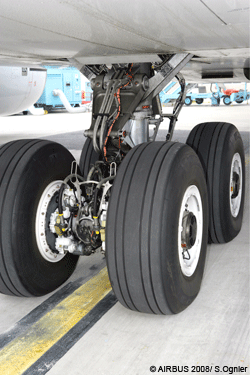
\includegraphics[height=4cm]{images/frein.png} \\
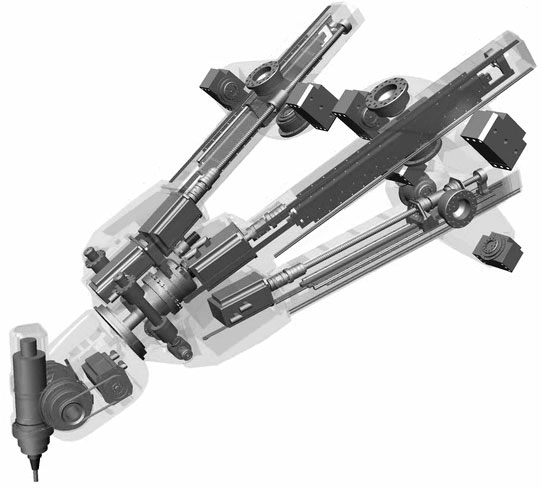
\includegraphics[height=4cm]{images/tripteor.png} \\ 
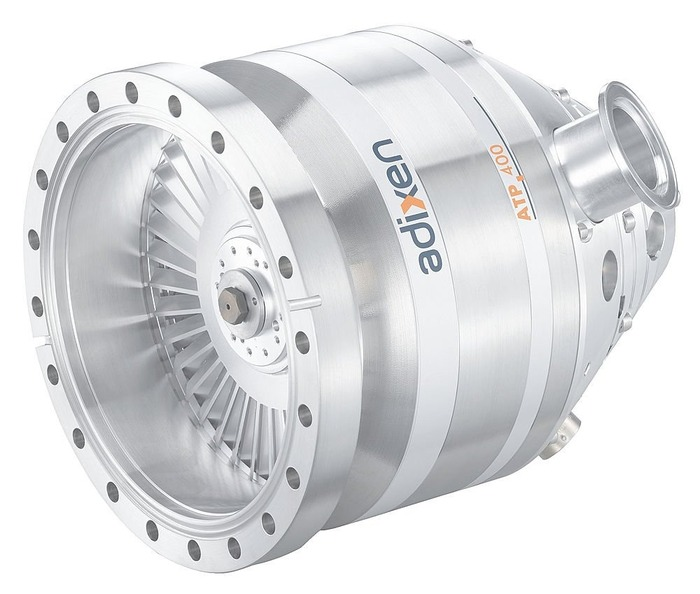
\includegraphics[height=4cm]{images/pompe.png} \\
\end{center}
}%figues de la page de garde
\def\xxpied{%
Partie 2 -- Découverte des SLCI\\
Ch. 2 : Transformées de Laplace -- \xxactivite%
}

%---------------------------------------------------------------------------


\begin{document}
\chapterimage{png/Fond_SLCI}
\pagestyle{empty}


%%%%%%%% PAGE DE GARDE COURS
\ifcours
\begin{tikzpicture}[remember picture,overlay]
\node at (current page.north west)
{\begin{tikzpicture}[remember picture,overlay]
\node[anchor=north west,inner sep=0pt] at (0,0) {\includegraphics[width=\paperwidth]{\thechapterimage}};
\draw[anchor=west] (-2cm,-8cm) node [line width=2pt,rounded corners=15pt,draw=ocre,fill=white,fill opacity=0.6,inner sep=40pt]{\strut\makebox[22cm]{}};
\draw[anchor=west] (1cm,-8cm) node {\huge\sffamily\bfseries\color{black} %
\begin{minipage}{1cm}
\rotatebox{90}{\LARGE\sffamily\textsc{\color{ocre}\textbf{\xxnumpartie}}}
\end{minipage} \hfill
\begin{minipage}[c]{14cm}
\begin{titrepartie}
\begin{flushright}
\renewcommand{\baselinestretch}{1.1} 
\Large\sffamily\textsc{\textbf{\xxpartie}}
\renewcommand{\baselinestretch}{1} 
\end{flushright}
\end{titrepartie}
\end{minipage} \hfill
\begin{minipage}[c]{3.5cm}
{\large\sffamily\textsc{\textbf{\color{ocre} \discipline}}}
\end{minipage} 
 };
\end{tikzpicture}};
\end{tikzpicture}


\begin{tikzpicture}[overlay]
\node[shape=rectangle, 
      rounded corners = .25 cm,
	  draw= ocre,
	  line width=2pt, 
	  fill = ocre!10,
	  minimum width  = 2.5cm,
	  minimum height = 3cm,] at (18cm,0) {};
\node at (17.7cm,0) {\rotatebox{90}{\textbf{\Large\color{ocre}{\classe}}}};
%{};
\end{tikzpicture}

\vspace{3.5cm}

\begin{tikzpicture}[remember picture,overlay]
\draw[anchor=west] (-2cm,-6cm) node {\huge\sffamily\bfseries\color{black} %
\begin{minipage}{2cm}
\begin{center}
\LARGE\sffamily\textsc{\color{ocre}\textbf{\xxactivite}}
\end{center}
\end{minipage} \hfill
\begin{minipage}[c]{15cm}
\begin{titrechapitre}
\renewcommand{\baselinestretch}{1.1} 
\Large\sffamily\textsc{\textbf{\xxnumchapitre}}

\Large\sffamily\textsc{\textbf{\xxchapitre}}
\vspace{.5cm}

\renewcommand{\baselinestretch}{1} 
\normalsize\normalfont
\xxcompetences
\end{titrechapitre}
\end{minipage}  };
\end{tikzpicture}
\vfill

\begin{flushright}
\begin{minipage}[c]{.3\linewidth}
\begin{center}
\xxfigures
\end{center}
\end{minipage}\hfill
\begin{minipage}[c]{.6\linewidth}
\startcontents
\printcontents{}{1}{}
\end{minipage}
\end{flushright}

\begin{tikzpicture}[remember picture,overlay]
\draw[anchor=west] (4.5cm,-.7cm) node {
\begin{minipage}[c]{.2\linewidth}
\begin{flushright}

\includegraphics[width=2cm]{png/logoCC}
\end{flushright}
\end{minipage}
\begin{minipage}[c]{.2\linewidth}
\textsl{\xxauteur} \\
\textsl{\classe}
\end{minipage}
 };
\end{tikzpicture}
\newpage
\pagestyle{fancy}

\newpage
\pagestyle{fancy}

\else
\fi


%%%%%%%% PAGE DE GARDE TD
\iftd
%\begin{tikzpicture}[remember picture,overlay]
%\node at (current page.north west)
%{\begin{tikzpicture}[remember picture,overlay]
%\draw[anchor=west] (-2cm,-3.25cm) node [line width=2pt,rounded corners=15pt,draw=ocre,fill=white,fill opacity=0.6,inner sep=40pt]{\strut\makebox[22cm]{}};
%\draw[anchor=west] (1cm,-3.25cm) node {\huge\sffamily\bfseries\color{black} %
%\begin{minipage}{1cm}
%\rotatebox{90}{\LARGE\sffamily\textsc{\color{ocre}\textbf{\xxnumpartie}}}
%\end{minipage} \hfill
%\begin{minipage}[c]{13.5cm}
%\begin{titrepartie}
%\begin{flushright}
%\renewcommand{\baselinestretch}{1.1} 
%\Large\sffamily\textsc{\textbf{\xxpartie}}
%\renewcommand{\baselinestretch}{1} 
%\end{flushright}
%\end{titrepartie}
%\end{minipage} \hfill
%\begin{minipage}[c]{3.5cm}
%{\large\sffamily\textsc{\textbf{\color{ocre} \discipline}}}
%\end{minipage} 
% };
%\end{tikzpicture}};
%\end{tikzpicture}

%%%%%%%%%% PAGE DE GARDE TD %%%%%%%%%%%%%%%
%\begin{tikzpicture}[overlay]
%\node[shape=rectangle, 
%      rounded corners = .25 cm,
%	  draw= ocre,
%	  line width=2pt, 
%	  fill = ocre!10,
%	  minimum width  = 2.5cm,
%	  minimum height = 2.5cm,] at (18.5cm,0) {};
%\node at (17.7cm,0) {\rotatebox{90}{\textbf{\Large\color{ocre}{\classe}}}};
%%{};
%\end{tikzpicture}

% PARTIE ET CHAPITRE
%\begin{tikzpicture}[remember picture,overlay]
%\draw[anchor=west] (-1cm,-2.1cm) node {\large\sffamily\bfseries\color{black} %
%\begin{minipage}[c]{15cm}
%\begin{flushleft}
%\xxnumchapitre \\
%\xxchapitre
%\end{flushleft}
%\end{minipage}  };
%\end{tikzpicture}

% Bandeau titre exo
\begin{tikzpicture}[remember picture,overlay]
\draw[anchor=west] (-2cm,-6cm) node {\huge\sffamily\bfseries\color{black} %
\begin{minipage}{5cm}
\begin{center}
\LARGE\sffamily\color{ocre}\textbf{\textsc{\xxactivite}}

\begin{center}
\xxfigures
\end{center}

\end{center}
\end{minipage} \hfill
\begin{minipage}[c]{12cm}
\begin{titrechapitre}
\renewcommand{\baselinestretch}{1.1} 
\large\sffamily\textbf{\textsc{\xxtitreexo}}

\small\sffamily{\textbf{\textit{\color{black!70}\xxsourceexo}}}
\vspace{.5cm}

\renewcommand{\baselinestretch}{1} 
\normalsize\normalfont
\xxcompetences
\end{titrechapitre}
\end{minipage}  };
\end{tikzpicture}

\else
\fi


%%%%%%%% PAGE DE GARDE FICHE
\iffiche
\begin{tikzpicture}[remember picture,overlay]
\node at (current page.north west)
{\begin{tikzpicture}[remember picture,overlay]
\draw[anchor=west] (-2cm,-3.25cm) node [line width=2pt,rounded corners=15pt,draw=ocre,fill=white,fill opacity=0.6,inner sep=40pt]{\strut\makebox[22cm]{}};
\draw[anchor=west] (1cm,-3.25cm) node {\huge\sffamily\bfseries\color{black} %
\begin{minipage}{1cm}
\rotatebox{90}{\LARGE\sffamily\textsc{\color{ocre}\textbf{\xxnumpartie}}}
\end{minipage} \hfill
\begin{minipage}[c]{14cm}
\begin{titrepartie}
\begin{flushright}
\renewcommand{\baselinestretch}{1.1} 
\large\sffamily\textsc{\textbf{\xxpartie} \\} 

\vspace{.2cm}

\normalsize\sffamily\textsc{\textbf{\xxnumchapitre -- \xxchapitre}}
\renewcommand{\baselinestretch}{1} 
\end{flushright}
\end{titrepartie}
\end{minipage} \hfill
\begin{minipage}[c]{3.5cm}
{\large\sffamily\textsc{\textbf{\color{ocre} \discipline}}}
\end{minipage} 
 };
\end{tikzpicture}};
\end{tikzpicture}


\begin{tikzpicture}[overlay]
\node[shape=rectangle, 
      rounded corners = .25 cm,
	  draw= ocre,
	  line width=2pt, 
	  fill = ocre!10,
	  minimum width  = 2.5cm,
	  minimum height = 2.5cm,] at (18.5cm,0.5cm) {};
%	  minimum height = 2.5cm,] at (18.5cm,0cm) {};
\node at (17.7cm,0.5) {\rotatebox{90}{\textsf{\textbf{\large\color{ocre}{\classe}}}}};
%{};
\end{tikzpicture}



\else
\fi





%\documentclass[11pt,oneside]{article}
%\usepackage[T1]{fontenc}
\usepackage[utf8]{inputenc}
%\DeclareUnicodeCharacter{00A0}{ }
\usepackage[adobe-utopia]{mathdesign}

\usepackage{amsmath}
\usepackage[francais]{babel}
\usepackage[dvips]{graphicx}
%\usepackage{here}
\usepackage{framed}
\usepackage[normalem]{ulem}
\usepackage{fancyhdr}
\usepackage{titlesec}
\usepackage{vmargin}

\usepackage{amsmath}
\usepackage{ifthen}
\usepackage{multirow}
\usepackage{multicol} % Portions de texte en colonnes

%\usepackage{xltxtra} % Logo XeLaTeX
%\usepackage{pst-solides3d}
\usepackage{color}
%\usepackage{colortbl}
\usepackage{titletoc} % Pour la mise en forme de la table des matières

%\usepackage[crop=off]{auto-pst-pdf}
%\usepackage{bclogo}


%\usepackage{longtable}
%\usepackage{flafter}%floatants après la référence
%\usepackage{pst-solides3d}
%\usepackage{pstricks}
%\usepackage{minitoc}
%\setcounter{minitocdepth}{4}
%\usepackage{draftcopy}% "Brouillon"
%\usepackage{floatflt}
%\usepackage{psfrag}
%\usepackage{listings} % Permet d'insérer du code de programmation
%\usepackage{lmodern}
%\usepackage[adobe-utopia,uppercase=upright,greeklowercase=upright]{mathdesign}
%\usepackage{minionpro}
%\usepackage{pifont}
%\usepackage{amssymb}
%\usepackage[francais]{varioref}

\setmarginsrb{1.5cm}{1cm}{1cm}{1.5cm}{1cm}{1cm}{1cm}{1cm}

\definecolor{gris25}{gray}{0.75}
\definecolor{bleu}{RGB}{18,33,98}
\definecolor{bleuf}{RGB}{42,94,171}
\definecolor{bleuc}{RGB}{231,239,247}
\definecolor{rougef}{RGB}{185,18,27}
\definecolor{rougec}{RGB}{255,230,231}
\definecolor{vertf}{RGB}{103,126,82}
\definecolor{vertc}{RGB}{220,255,191}
\definecolor{violetf}{RGB}{112,48,160}
\definecolor{violetc}{RGB}{230,224,236}
\definecolor{jaunec}{RGB}{220,255,191}
%%\usepackage{algorithm}
%\usepackage{algorithmic}
\usepackage[french]{algorithm2e}

\SetKwBlock{Fonction}{Début Fonction}{Fin Fonction}
\SetKwComment{Comment}{start}{end}
% Python sources

\usepackage{listings}
\lstloadlanguages{R}   % pour regler les pb d accent utf8 dans les codes
\lstset{language=R} % pour regler les pb d accent utf8 dans les codes

\usepackage{textcomp}
\usepackage{setspace}
%\usepackage{palatino}

%\usepackage{color}
\definecolor{Bleu}{rgb}{0.1,0.1,1.0}
\definecolor{Noir}{rgb}{0,0,0}
\definecolor{Grau}{rgb}{0.5,0.5,0.5}
\definecolor{DunkelGrau}{rgb}{0.15,0.15,0.15}
\definecolor{Hellbraun}{rgb}{0.5,0.25,0.0}
\definecolor{Magenta}{rgb}{1.0,0.0,1.0}
\definecolor{Gris}{gray}{0.5}
\definecolor{Vert}{rgb}{0,0.5,0}
\definecolor{SourceHintergrund}{rgb}{1,1.0,0.95}


%
\renewcommand{\lstlistlistingname}{Listings}
\renewcommand{\lstlistingname}{Listing}

\lstnewenvironment{python}[1][]{
\lstset{
%escapeinside={\%*}{*)},
%inputencoding=utf8,   % pour regler les pb d accent utf8 dans les codes
%extendedchars=true,   % pour regler les pb d accent utf8 dans les codes
language=python,
basicstyle=\sffamily\footnotesize, 	
stringstyle=\color{red}, 
showstringspaces=false, 
alsoletter={1234567890},
otherkeywords={\ , \}, \{},
keywordstyle=\color{blue},
emph={access,and,break,class,continue,def,del,elif ,else,
except,exec,finally,for,from,global,if,import,in,i s,
lambda,not,or,pass,print,raise,return,try,while},
emphstyle=\color{black}\bfseries,
emph={[2]True, False, None, self},
emphstyle=[2]\color{green},
emph={[3]from, import, as},
emphstyle=[3]\color{blue},
upquote=true,
columns=flexible, % pour empecher d'avoir un espacement mono
morecomment=[s]{"""}{"""},
commentstyle=\color{Hellbraun}\slshape, 
%emph={[4]1, 2, 3, 4, 5, 6, 7, 8, 9, 0},
emphstyle=[4]\color{blue},
literate=*{:}{{\textcolor{blue}:}}{1}
{=}{{\textcolor{blue}=}}{1}
{-}{{\textcolor{blue}-}}{1}
{+}{{\textcolor{blue}+}}{1}
{*}{{\textcolor{blue}*}}{1}
{!}{{\textcolor{blue}!}}{1}
{(}{{\textcolor{blue}(}}{1}
{)}{{\textcolor{blue})}}{1}
{[}{{\textcolor{blue}[}}{1}
{]}{{\textcolor{blue}]}}{1}
{<}{{\textcolor{blue}<}}{1}
{>}{{\textcolor{blue}>}}{1}
{COMPLETER}{{\textcolor{red}COMPLETER}}{1},
literate=%
            {é}{{\'{e}}}1
            {è}{{\`{e}}}1
            {ê}{{\^{e}}}1
            {ë}{{\¨{e}}}1
            {û}{{\^{u}}}1
            {ù}{{\`{u}}}1
            {â}{{\^{a}}}1
            {à}{{\`{a}}}1
            {î}{{\^{i}}}1
            {ç}{{\c{c}}}1
            {Ç}{{\c{C}}}1
            {É}{{\'{E}}}1
            {Ê}{{\^{E}}}1
            {À}{{\`{A}}}1
            {Â}{{\^{A}}}1
            {Î}{{\^{I}}}1, % pour regler les pb d accent utf8 dans les codes
%framexleftmargin=1mm, framextopmargin=1mm, frame=shadowbox, rulesepcolor=\color{blue},#1
%backgroundcolor=\color{SourceHintergrund}, 
%framexleftmargin=1mm, framexrightmargin=1mm, framextopmargin=1mm, frame=single, framerule=1pt, rulecolor=\color{black},#1
}}{}



\lstnewenvironment{scilab}[1][]{
\lstset{
language=scilab,
basicstyle=\sffamily\footnotesize, 	
stringstyle=\color{red}, 
showstringspaces=false, 
alsoletter={1234567890},
otherkeywords={\ , \}, \{},
keywordstyle=\color{blue},
emph={access,and,break,class,continue,def,del,elif ,else,
except,exec,finally,for,from,global,if,import,in,i s,
lambda,not,or,pass,print,raise,return,try,while,Debut},
emphstyle=\color{black}\bfseries,
emph={[2]True, False, None, self},
emphstyle=[2]\color{green},
emph={[3]from, import, as},
emphstyle=[3]\color{blue},
upquote=true,
columns=flexible, % pour empecher d'avoir un espacement mono
morecomment=[s]{"""}{"""},
commentstyle=\color{Hellbraun}\slshape, 
%emph={[4]1, 2, 3, 4, 5, 6, 7, 8, 9, 0},
emphstyle=[4]\color{blue},
literate=*{:}{{\textcolor{blue}:}}{1}
{=}{{\textcolor{blue}=}}{1}
{-}{{\textcolor{blue}-}}{1}
{+}{{\textcolor{blue}+}}{1}
{*}{{\textcolor{blue}*}}{1}
{!}{{\textcolor{blue}!}}{1}
{(}{{\textcolor{blue}(}}{1}
{)}{{\textcolor{blue})}}{1}
{[}{{\textcolor{blue}[}}{1}
{]}{{\textcolor{blue}]}}{1}
{<}{{\textcolor{blue}<}}{1}
{>}{{\textcolor{blue}>}}{1},
%framexleftmargin=1mm, framextopmargin=1mm, frame=shadowbox, rulesepcolor=\color{blue},#1
%backgroundcolor=\color{SourceHintergrund}, 
%framexleftmargin=1mm, framexrightmargin=1mm, framextopmargin=1mm, frame=single, framerule=1pt, rulecolor=\color{black},#1
}}{}


\lstdefinestyle{stylepython}{%
escapeinside={\%*}{*)},
inputencoding=utf8,   % pour regler les pb d accent utf8 dans les codes
extendedchars=true,   % pour regler les pb d accent utf8 dans les codes
language=python,
basicstyle=\sffamily\footnotesize, 	
stringstyle=\color{red}, 
showstringspaces=false, 
alsoletter={1234567890},
otherkeywords={\ , \}, \{},
keywordstyle=\color{blue},
emph={access,and,break,class,continue,def,del,elif ,else,
except,exec,finally,for,from,global,if,import,in,i s,
lambda,not,or,pass,print,raise,return,try,while},
emphstyle=\color{black}\bfseries,
emph={[2]True, False, None, self},
emphstyle=[2]\color{green},
emph={[3]from, import, as},
emphstyle=[3]\color{blue},
upquote=true,
columns=flexible, % pour empecher d'avoir un espacement mono
morecomment=[s]{"""}{"""},
commentstyle=\color{Hellbraun}\slshape, 
%emph={[4]1, 2, 3, 4, 5, 6, 7, 8, 9, 0},
emphstyle=[4]\color{blue},
literate=*{:}{{\textcolor{blue}:}}{1}
{=}{{\textcolor{blue}=}}{1}
{-}{{\textcolor{blue}-}}{1}
{+}{{\textcolor{blue}+}}{1}
{*}{{\textcolor{blue}*}}{1}
{!}{{\textcolor{blue}!}}{1}
{(}{{\textcolor{blue}(}}{1}
{)}{{\textcolor{blue})}}{1}
{[}{{\textcolor{blue}[}}{1}
{]}{{\textcolor{blue}]}}{1}
{<}{{\textcolor{blue}<}}{1}
{>}{{\textcolor{blue}>}}{1}
{COMPLETER}{{\textcolor{red}COMPLETER}}{1},
literate=%
            {é}{{\'{e}}}1
            {è}{{\`{e}}}1
            {ê}{{\^{e}}}1
            {ë}{{\¨{e}}}1
            {û}{{\^{u}}}1
            {ù}{{\`{u}}}1
            {â}{{\^{a}}}1
            {à}{{\`{a}}}1
            {î}{{\^{i}}}1
            {ç}{{\c{c}}}1
            {Ç}{{\c{C}}}1
            {É}{{\'{E}}}1
            {Ê}{{\^{E}}}1
            {À}{{\`{A}}}1
            {Â}{{\^{A}}}1
            {Î}{{\^{I}}}1,
%numbers=left,                    % where to put the line-numbers; possible values are (none, left, right)
%numbersep=5pt,                   % how far the line-numbers are from the code
%numberstyle=\tiny\color{mygray}, % the style that is used for the line-numbers
}

%
%\renewcommand{\algorithmicrequire} {\textbf{\textsc{Entrées:}}}
%\renewcommand{\algorithmicensure}  {\textbf{\textsc{Sorties:}}}
%\renewcommand{\algorithmicwhile}   {\textbf{tantque}}
%\renewcommand{\algorithmicdo}      {\textbf{faire}}
%\renewcommand{\algorithmicendwhile}{\textbf{fin tantque}}
%\renewcommand{\algorithmicend}     {\textbf{fin}}
%\renewcommand{\algorithmicif}      {\textbf{si}}
%\renewcommand{\algorithmicendif}   {\textbf{finsi}}
%\renewcommand{\algorithmicelse}    {\textbf{sinon}}
%\renewcommand{\algorithmicthen}    {\textbf{alors}}
%\renewcommand{\algorithmicfor}     {\textbf{pour}}
%\renewcommand{\algorithmicforall}  {\textbf{pour tout}}
%\renewcommand{\algorithmicdo}      {\textbf{faire}}
%\renewcommand{\algorithmicendfor}  {\textbf{fin pour}}
%\renewcommand{\algorithmicloop}    {\textbf{boucler}}
%\renewcommand{\algorithmicendloop} {\textbf{fin boucle}}
%\renewcommand{\algorithmicrepeat}  {\textbf{répéter}}
%\renewcommand{\algorithmicuntil}   {\textbf{jusqu'à}}

\lstnewenvironment{termi}[1][]{
\lstset{
language=scilab,
basicstyle=\sffamily\footnotesize, 	
stringstyle=\color{red}, 
showstringspaces=false, 
alsoletter={1234567890},
otherkeywords={\ , \}, \{},
keywordstyle=\color{blue},
emph={access,and,break,class,continue,def,del,elif ,else,
except,exec,finally,for,from,global,if,import,in,i s,
lambda,not,or,pass,print,raise,return,try,while,Debut},
emphstyle=\color{black}\bfseries,
emph={[2]True, False, None, self},
emphstyle=[2]\color{green},
emph={[3]from, import, as},
emphstyle=[3]\color{blue},
upquote=true,
columns=flexible, % pour empecher d'avoir un espacement mono
morecomment=[s]{"""}{"""},
commentstyle=\color{Hellbraun}\slshape, 
%emph={[4]1, 2, 3, 4, 5, 6, 7, 8, 9, 0},
emphstyle=[4]\color{blue},
literate=*{:}{{\textcolor{blue}:}}{1}
{=}{{\textcolor{blue}=}}{1}
{-}{{\textcolor{blue}-}}{1}
{+}{{\textcolor{blue}+}}{1}
{*}{{\textcolor{blue}*}}{1}
{!}{{\textcolor{blue}!}}{1}
{(}{{\textcolor{blue}(}}{1}
{)}{{\textcolor{blue})}}{1}
{[}{{\textcolor{blue}[}}{1}
{]}{{\textcolor{blue}]}}{1}
{<}{{\textcolor{blue}<}}{1}
{>}{{\textcolor{blue}>}}{1},
%framexleftmargin=1mm, framextopmargin=1mm, frame=shadowbox, rulesepcolor=\color{blue},#1
%backgroundcolor=\color{SourceHintergrund}, 
%framexleftmargin=1mm, framexrightmargin=1mm, framextopmargin=1mm, frame=single, framerule=1pt, rulecolor=\color{black},#1
}}{}


%
%\renewcommand{\algorithmicrequire} {\textbf{\textsc{Entrées:}}}
%\renewcommand{\algorithmicensure}  {\textbf{\textsc{Sorties:}}}
%\renewcommand{\algorithmicwhile}   {\textbf{tantque}}
%\renewcommand{\algorithmicdo}      {\textbf{faire}}
%\renewcommand{\algorithmicendwhile}{\textbf{fin tantque}}
%\renewcommand{\algorithmicend}     {\textbf{fin}}
%\renewcommand{\algorithmicif}      {\textbf{si}}
%\renewcommand{\algorithmicendif}   {\textbf{finsi}}
%\renewcommand{\algorithmicelse}    {\textbf{sinon}}
%\renewcommand{\algorithmicthen}    {\textbf{alors}}
%\renewcommand{\algorithmicfor}     {\textbf{pour}}
%\renewcommand{\algorithmicforall}  {\textbf{pour tout}}
%\renewcommand{\algorithmicdo}      {\textbf{faire}}
%\renewcommand{\algorithmicendfor}  {\textbf{fin pour}}
%\renewcommand{\algorithmicloop}    {\textbf{boucler}}
%\renewcommand{\algorithmicendloop} {\textbf{fin boucle}}
%\renewcommand{\algorithmicrepeat}  {\textbf{répéter}}
%\renewcommand{\algorithmicuntil}   {\textbf{jusqu'à}}
%
%
%%Si le boolen xp est vrai : compilation pour xabi
%%Sinon compilation Damien
%\newboolean{xp}
%\setboolean{xp}{true}
%
%\newboolean{prof}
%\setboolean{prof}{true}
%
%\def\xxtitre{\ifthenelse{\boolean{xp}}{
%CI 2 -- SLCI : Étude du comportement des Systèmes Linéaires Continus Invariants}{}}
%
%\def\xxsoustitre{\ifthenelse{\boolean{xp}}{
%Chapitre 2 -- Modélisation des Systèmes Linéaires Continus Invariants -- Transformée de Laplace}{}}
%
%\def\xxauteur{\ifthenelse{\boolean{xp}}{
%\noindent 2013 -- 2014 \\
%Xavier \textsc{Pessoles}}{
%Damien Iceta}}
%
%
%\def\xxpied{\ifthenelse{\boolean{xp}}{
%CI 2 : SLCI -- Cours \\
%Ch 2 : Modélisation des SLCI -- \ifthenelse{\boolean{prof}}{P}{E}%
%}{
%TD -- CI 3 : Ingénierie numérique et simulation}}
%
%
%
%\ifthenelse{\boolean{xp}}{
%\usepackage[%
%    pdftitle={SLCI - Modélisation des SLCI},
%    pdfauthor={Xavier Pessoles},
%    colorlinks=true,
%    linkcolor=blue,
%    citecolor=magenta]{hyperref}}{
%\usepackage[%
%    pdftitle={OS et Environnement de développement},
%    pdfauthor={Damien Iceta},
%    colorlinks=true,
%    linkcolor=blue,
%    citecolor=magenta]{hyperref}}
%
%
%
%\usepackage{pifont}
%\sloppy
%\hyphenpenalty 10000
%
%\begin{document}
%
%
%



% \makeatletter \let\ps@plain\ps@empty \makeatother
%% DEBUT DU DOCUMENT
%% =================




%------------- En tetes et Pieds de Pages ------------


\pagestyle{fancy}
\ifthenelse{\boolean{xp}}{%
\renewcommand{\headrulewidth}{0pt}}{%
\renewcommand{\headrulewidth}{0.2pt}} %pour mettre le trait en haut
%\renewcommand{\headrulewidth}{0.2pt}

\fancyhead{}
\fancyhead[L]{%
\ifthenelse{\boolean{xp}}{%
\noindent\begin{minipage}[c]{2.6cm}%

\includegraphics[width=2cm]{png/logo_ptsi.png}%
\end{minipage}%
}{%
\footnotesize{\textit{\textsf{Lycée François Premier}}}
}}

\ifthenelse{\boolean{xp}}{%
\fancyhead[C]{\rule{12cm}{.5pt}}}{
}


\fancyhead[R]{%
\noindent\begin{minipage}[c]{3cm}
\begin{flushright}
\footnotesize{\textit{\textsf{Sciences Industrielles \\ de l'ingénieur}}}%
\end{flushright}
\end{minipage}
}


\ifthenelse{\boolean{xp}}{%
\fancyhead[C]{\rule{12cm}{.5pt}}}{
}

\renewcommand{\footrulewidth}{0.2pt}

\fancyfoot[C]{\footnotesize{\bfseries \thepage}}
\fancyfoot[L]{%
\begin{minipage}[c]{.2\linewidth}
\noindent\footnotesize{{\xxauteur}}
\end{minipage}
\ifthenelse{\boolean{xp}}{}{%
\begin{minipage}[c]{.15\linewidth}

\includegraphics[width=2cm]{png/logoCC.png}
\end{minipage}}
}


\fancyfoot[R]{\footnotesize{\xxpied}}


%
%\begin{center}
% \huge\textsc{\xxtitre}
%\end{center}
%
%\begin{center}
% \LARGE\textsc{\xxsoustitre}
%\end{center}
%
%
%
%
%\vspace{.5cm}
%
%
%\begin{center}
%\begin{tabular}{ccccc}
%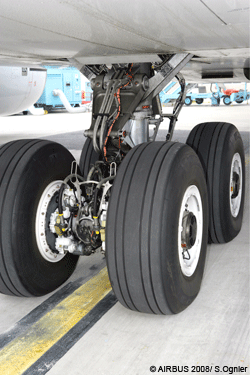
\includegraphics[height=4cm]{images/frein.png} &&
%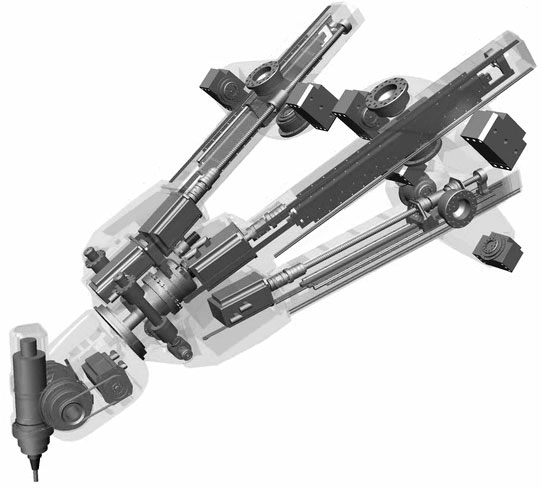
\includegraphics[height=4cm]{images/tripteor.png} &&
%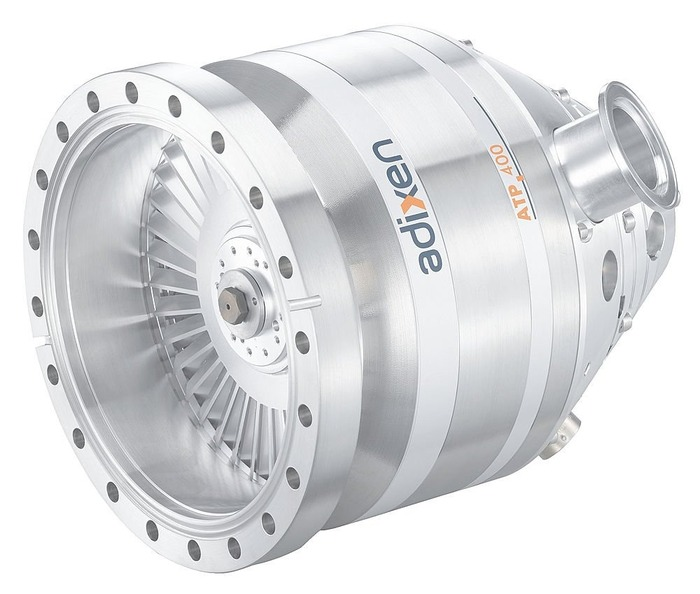
\includegraphics[height=4cm]{images/pompe.png} \\
%\textit{Asservissement du freinage} &&
%\textit{Asservissement en } &&
%\textit{Asservissement de } \\
%\textit{d'un A 318} &&
%\textit{vitesse et position} &&
%\textit{la position du rotor} \\
%&&
%\textit{d'un centre d'usinage} && 
%\textit{d'une pompe turbo moléculaire} 
%\end{tabular}
%\end{center}
%
%
%
%
%
%\vspace{.2cm}
%Il est possible prévoir le comportement de systèmes intégrant des technologies différentes. Par exemple, en mode automatique, le freinage d'un avion dépend de son accélération (technologie mécanique). L'envoi de l'ordre de freinage est piloté par une servo-valve électro-hydraulique (technologies électriques et hydrauliques).
%
%Il va donc falloir d'une part définir des outils mathématiques indépendant des différentes technologies pour décrire le fonctionnement des systèmes. D'autre part, ces modèles devront permettre de connaître les réponses du système en fonction de sollicitations diverses (échelons, rampes, sinusoïdes ...).
%
%
%Classiquement, ces systèmes sont modélisables par des équations différentielles. Or, déterminer une solution analytique pour une équation différentielle n'est pas toujours aisé.
%
%\begin{obj}
%\textsc{Problématiques :}
%\begin{itemize}
%\item Comment modéliser un système dont le fonctionnement fait appel à plusieurs champs de la physiques ?
%\item Comment déterminer le comportement d'un système lorsque celui-ci est régit par une équation différentielle complexe ?
%\end{itemize}
%\end{obj}
%
%\begin{rem}
%\textsc{Savoirs :}
%\begin{itemize}
%\item Mod-C2.1	Modélisation par équations différentielles.
%\item Mod-C2.2	Représentation par fonction de transfert (formalisme de Laplace).
%\end{itemize}
%\end{rem}
%
%
%
%\setlength{\parskip}{0ex plus 0.2ex minus 0ex}
% \renewcommand{\contentsname}{}
% \renewcommand{\baselinestretch}{1}
%
%% \vspace{1cm}
%\textit{Ce document est en évolution permanente. Merci de signaler toutes
%erreurs ou coquilles.}
%
%\tableofcontents
%
% \renewcommand{\baselinestretch}{1.2}
%\setlength{\parskip}{2ex plus 0.5ex minus 0.2ex}

Les notions mathématiques abordées dans ce chapitre n'ont pas pour but de se substituer à un cours de mathématiques mais de donner des propriétés et des définitions utiles pour l'étude des systèmes continus linéaires invariants.

\section{Modélisation d'un système par équations différentielles}
\subsection{Modélisation d'un filtre du premier ordre}

\begin{minipage}[c]{.6\linewidth}
On considère le circuit électrique ci-contre. On cherche à connaître le comportement du système vis à vis de différents types de signaux.
\end{minipage}\hfill
\begin{minipage}[c]{.35\linewidth}
\begin{center}
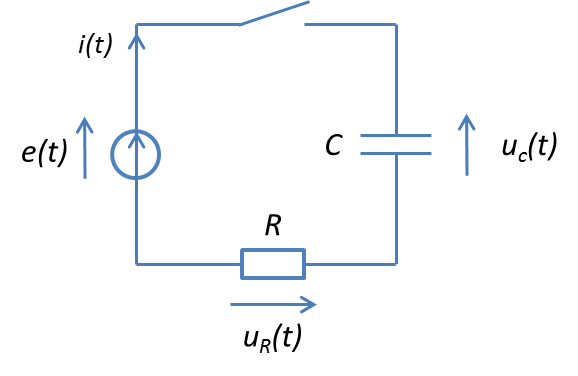
\includegraphics[width=.9\textwidth]{images/RC}
\end{center}
\end{minipage}

D'après la loi des mailles, on a :
$$
e(t)=u_R(t) + u_C(t)
$$

Connaissant la relation de comportement aux bornes d'un condensateur ($i(t)=C\dfrac{du_c}{dt}$)et d'une résistance ($u_R(t)=R\cdot i(t)$)on a donc :
$$
e(t)=R\cdot i(t) +  u_C(t) 
%\Longleftrightarrow e(t)=R\cdot \dfrac{dq(t)}{dt} +  u_C(t)
\Longleftrightarrow e(t)=R\cdot C\cdot \dfrac{du_C(t)}{dt} +  u_C(t)
$$

On cherche donc à résoudre l'équation différentielle suivante : 

$$
\dfrac{du_C(t)}{dt} +  \dfrac{1}{RC}u_C(t) = \dfrac{1}{RC}e(t)
$$

On cherche la réponse du système lorsque $e(t)$ est une fonction échelon définie ainsi :
$$\left\{
\begin{array}{l}
e(t)=0 \text{ si t<0}\\
e(t)=E_0 \text{ sinon}\\
\end{array}
\right.
$$

\subparagraph*{Recherche d'une solution particulière de l'équation complète}
$s_p(t)=E_0$ est une solution particulière de l'équation complète.

\subparagraph*{Recherche d'une solution générale de l'équation sans second membre}
$s_g(t)$ est de la forme $s_g(t)=\alpha e^{ - \dfrac{1}{RC} t}$ où $\alpha \in \mathbb{R}$.


\subparagraph*{Résolution de l'équation différentielle}
On a donc  
$$ u_C(t)=s_p(t) + s_g(t) =E_0 + \alpha  e^{-\dfrac{1}{RC}t}
$$

A $t=0$, le condensateur est déchargé. On a donc en $t=0$: 
$$ 
u_C(0)=0 \Longleftrightarrow E_0 + \alpha   = 0 \Longleftrightarrow \alpha  = -E_0    
$$
On a donc :
$$ u_C(t) = E_0 -E_0 e^{-\dfrac{1}{RC}t}
$$


\subsection{Modélisation d'un système du second ordre}

\begin{minipage}[c]{.6\linewidth}
On considère le circuit électrique ci-contre. On cherche à connaître le comportement du système lors du déchargement du condensateur dans la bobine.
\end{minipage}\hfill
\begin{minipage}[c]{.35\linewidth}
\begin{center}
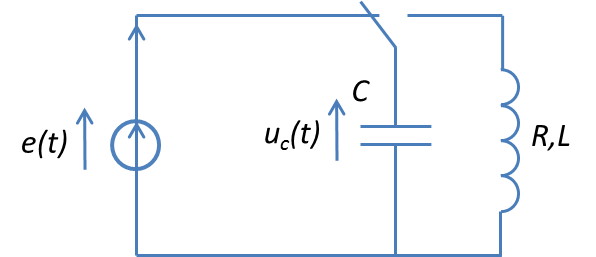
\includegraphics[width=.9\textwidth]{images/RLC}
\end{center}
\end{minipage}

D'après la loi des mailles, la loi de comportement de la tension aux bornes d'un condensateur, la loi d'Ohm et la loi de Faraday, on a : 
$$
u_C(t)-u_L(t)-u_R(t)=0 
\Longleftrightarrow u_C(t) - L\dfrac{di(t)}{dt} -Ri(t)=0 
\Longleftrightarrow u_C(t) + LC\dfrac{d^2u_C(t)}{dt^2} +RC \dfrac{du_C(t)}{dt}=0 
$$


Afin de savoir le comportement du système, il faut donc étudier l'équation différentielle suivante :  
$$
\dfrac{d^2u_C(t)}{dt^2} +\dfrac{R}{L} \dfrac{du_C(t)}{dt} + \dfrac{1}{LC}u_C(t)=0 
$$

\subparagraph*{Résolution de l'équation homogène et de l'équation différentielle}
L'équation homogène associée à cette équation est de la forme : 
$$
\lambda^2 +\dfrac{R}{L} \lambda + \dfrac{1}{LC}=0 
$$
Le discriminant vaut : 
$$
\Delta = \dfrac{R^2}{L^2}-4\dfrac{1}{LC}
$$

Suivant le signe de $\Delta$, on peut alors déterminer la solution de l'équation différentielle...


\begin{obj}
Avec la complexité croissante des systèmes, il devient de plus en plus difficile de trouver directement des solutions aux équations différentielles qui traduisent le comportement des systèmes. En SII, la résolution directe des équations différentielles ne sera jamais demandée.
\end{obj}

\subsection{Équation différentielle généralisée}
Lorsque le système se complexifie, on peut alors obtenir une équation différentielle qui régit la sortie du système $s(t)$ en fonction de l'entrée $e(t)$. La forme générale d'une équation différentielle d'ordre $n$ est donnée par :
$$
a_0 \cdot s(t)  + \sum\limits_{i=1}^n a_i \cdot \dfrac{d^i s(t)}{dt}
= b_0 \cdot e(t)  + \sum\limits_{i=1}^m  b_i \cdot\dfrac{d^i s(t)}{dt}
$$

\begin{rem}
Les systèmes étudiés impliqueront que $n\geq m$.
\end{rem}

Deux problèmes peuvent alors se poser :
\begin{itemize}
\item il n'existe pas toujours de solution simple et analytique pour les équations différentielles, notamment lorsque l'ordre est supérieur à 2;
\item il est difficile de résoudre ces équations en particulier lorsqu'on va chercher à modifier le type d'entrée.
\end{itemize}

L'outil mathématique qui va nous permettre d'analyser le comportement de systèmes complexes asservis est la transformation de Laplace. Cette transformation va nous permettre de passer d'une équation différentielle à une équation polynomiale, plus aisée à manipuler :
$$
  S(p) \cdot  \sum\limits_{i=0}^n c_i p^i
= E(p) \cdot  \sum\limits_{i=0}^m d_i p^i
$$
Dans le domaine temporel, la variable est le temps, noté $t$. Dans le domaine de Laplace, la variable est notée $p$ (ou $s$ dans les pays anglo-saxons).

\begin{minipage}[c]{.45\linewidth}
\begin{center}
\textbf{Méthode de résolution d'une équation du second ordre dans le domaine temporel}
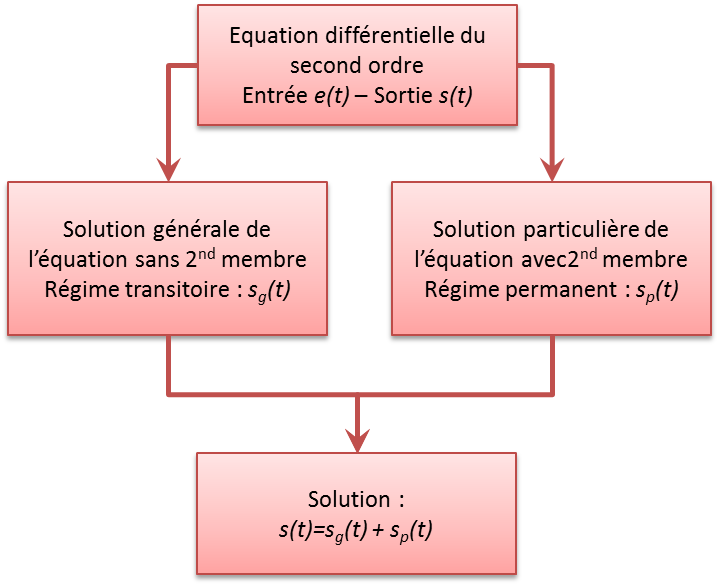
\includegraphics[width=\textwidth]{images/temporel}
\end{center}
\end{minipage} \hfill
\begin{minipage}[c]{.45\linewidth}
\begin{center}
\textbf{Méthode de résolution d'une équation dans le domaine de Laplace}
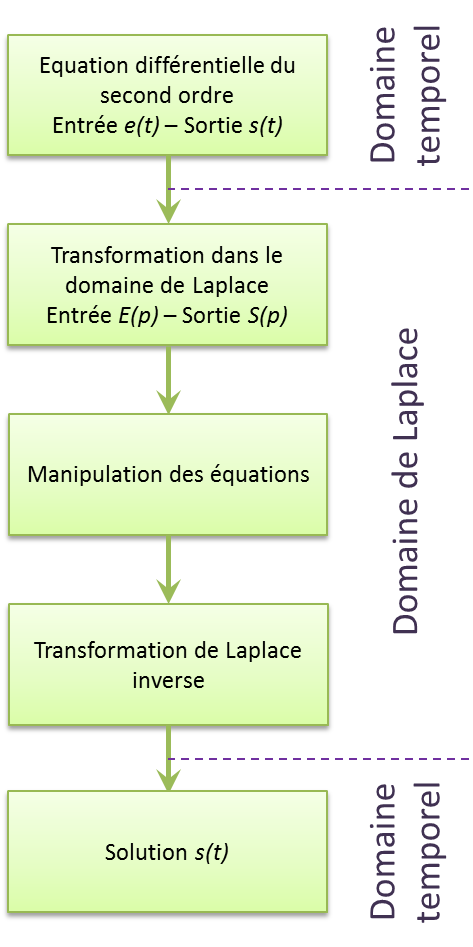
\includegraphics[width=.7\textwidth]{images/laplace}
\end{center}
\end{minipage} \hfill

\section{Propriétés des systèmes asservis}
\subsection{Systèmes linéaires}
\begin{defi}
\textbf{Système linéaire}

Soit un système d'entrée $e(t)$ et de sortie $s(t)$ caractérisé par sa fonction $F$ telle que $F(e(t))=s(t)$. Le système est dit linéaire s'il satisfait les conditions suivantes : 
\begin{itemize}
\item il est proportionnel : $\forall k \in \mathbb{R}$, $F(k\cdot e(t))=k\cdot s(t)$;
\item il obéit au principe de superposition : $F(e_1(t)+e_2(t))=s_1(t)+s_2(t)$.
\end{itemize}
\end{defi}

\begin{center}
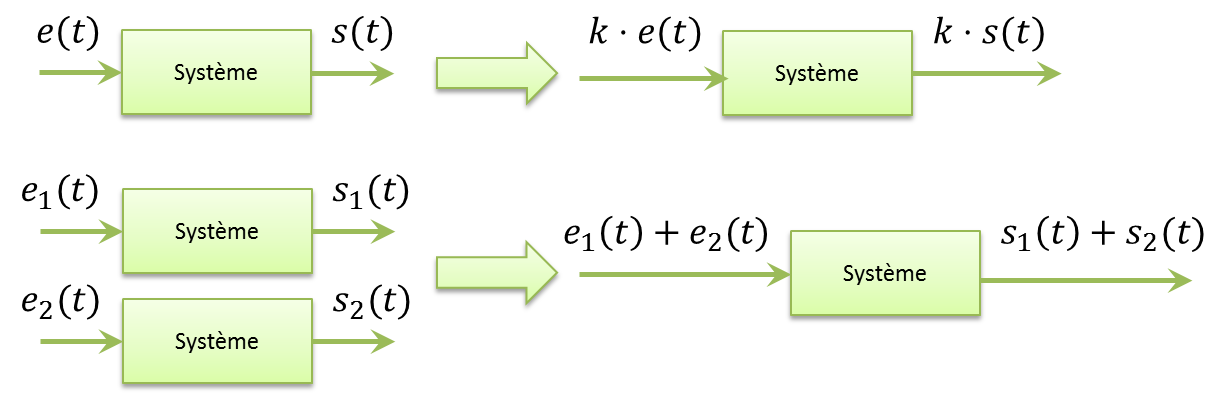
\includegraphics[width=.7\textwidth]{images/lineaire}
\end{center}

\subsection{Systèmes continus}
Un système est \textbf{continu}, par opposition à un système \textbf{discret} (ou
échantillonné, ou numérique), si les grandeurs physiques le caractérisant sont
des fonctions continues du temps. On parle aussi de systèmes
\textbf{analogiques}. 

La plupart des systèmes physiques, du point de vue macroscopique, sont
continus. En revanche, un système informatique a besoin d'un temps non nul pour
réaliser un traitement de l'information. On ne peut donc pas le qualifier de
système continu. Il ne peut que traiter des valeurs prises sur des échantillons
de signaux constants qui lui sont soumis. On parle alors de système
échantillonné.

\subsection{Systèmes invariants}
\begin{defi}
\textbf{Système invariant}

Un système est invariant lorsque les relations entre l'entrée et la sortie ne
se modifient pas au cours du temps. Le système ne vieillit pas. 

Ainsi, $\forall T \in \mathbb{R}$ :
$$
F(e(t+T))=s(t+T)
$$
\end{defi}

\begin{center}
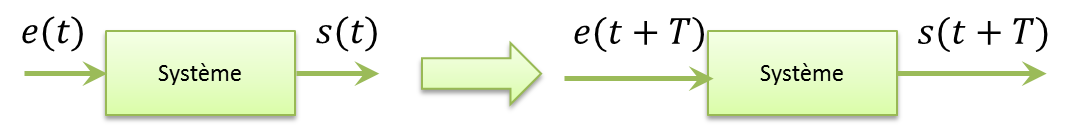
\includegraphics[width=.7\textwidth]{images/invariant}
\end{center}

\subsection{Systèmes non linéaires}
On peut vérifier la linéarité des systèmes en traçant sur un graphe l'entrée en abscisse et la sortie en ordonnée. Le système est linéaire si la courbe tracée est une droite passant par l'origine du repère.

Certains comportements physiques des systèmes ne sont pas linéaires :
\begin{itemize}
\item les phénomènes d'hystérésis;
\item les phénomènes de saturation;
\item les phénomènes de seuil;
\item ...
\end{itemize}

Les outils que nous développerons par la suite ne sont pas capable de modéliser ces phénomènes. Dans le cas où il faudrait impérativement modéliser ces comportements, il faudrait les linéariser autour des points de comportements.



\section{Transformée de Laplace}
\subsection{Définition}
\begin{defi}
\textbf{Transformée de Laplace}

À toute fonction du temps $f(t)$, nulle pour $t\leq0$ (fonction causale), on fait correspondre une fonction $F(p)$ de la variable complexe $p$ telle que :

\ifthenelse{\boolean{prof}}{%
$$
\mathcal{L}\left[f(t)\right] = F(p)=\int\limits_{0^{+}}^\infty f(t)e^{-pt}dt
$$}{
\rotatebox{90}{
\begin{tabular}{p{2cm}}
\\
\end{tabular}}
}

On note $\mathcal{L}\left[f(t)\right]$ la transformée directe et $\mathcal{L}^{-1}\left[F(p)\right]$ la transformée inverse.
\end{defi}

La transformée de Laplace permet de passer du domaine temporel au domaine dit de Laplace.

La variable $p$ (ou $s$) est un nombre complexe. On pose parfois $p=\sigma + j\omega$.

\begin{rem}
\textbf{Notation}

De manière générale, une fonction temporelle est nommée avec une lettre minuscule et sa transformée de Laplace avec une lettre majuscule. Dans le cas où la fonction temporelle est déjà une lettre majuscule, on conserve la même lettre. On a donc, par exemple : 
\begin{multicols}{2}
\begin{itemize}
\item $\mathcal{L}\left[f(t)\right] = F(p)$
\item $\mathcal{L}\left[e(t)\right] = E(p)$
\item $\mathcal{L}\left[s(t)\right] = S(p)$
\item $\mathcal{L}\left[C(t)\right] = C(p)$
\item $\mathcal{L}\left[\omega(t)\right] = \Omega(p)$
\item $\mathcal{L}\left[\theta(t)\right] = \Theta(p)$ ...
\end{itemize}
\end{multicols}
\end{rem}

%\begin{prop}
\textbf{Unicité}

\begin{itemize}
\item La transformée de Laplace de $f(t)$ est unique.
\item La transformée de Laplace inverse de $F(p)$ est unique.
\end{itemize}

%\end{prop}


\begin{exemple}
\textbf{Calcul de $\mathcal{L}\left[f(t) \right]$ avec $f(t)=k\quad \forall t> 0$ et $k\in \mathbb{R}$.}

\ifthenelse{\boolean{prof}}{%
\begin{eqnarray*}
\mathcal{L}\left[f(t) \right] 
= \mathcal{L}\left[k \right] 
= \int\limits_{0^{+}}^{+ \infty} k\cdot e^{-pt}dt
= k\cdot  \int\limits_{0^{+}}^{+ \infty}  e^{-pt}dt
= k \left[-\dfrac{1}{p} e^{-pt}\right]_{0^{+}}^{+\infty}
=\dfrac{k}{p}
\end{eqnarray*}

Ainsi $\mathcal{L}\left[k \right]=\dfrac{k}{p}$.

Dans la pratique la transformée de Laplace des fonctions usuelles ne se recalculera pas. Il faudra les connaître par c\oe{}ur.
}{
\rotatebox{90}{
\begin{tabular}{p{7cm}}
\\
\end{tabular}}
}



\end{exemple}




\subsection{Propriétés des transformées de Laplace}

%\begin{prop}
\textbf{Linéarité}

Soit $\mathcal{L}\left[f(t)\right] = F(p)$ et $\mathcal{L}\left[g(t)\right] =
G(p)$.

On démontre que :
$$\mathcal{L}\left[f(t) + g(t)\right] = 
\mathcal{L}\left[f(t)\right] +\mathcal{L}\left[g(t)\right] = F(p)+G(p)$$

et que :
$$\mathcal{L}\left[K\cdot f(t)\right] = K\cdot \mathcal{L}\left[f(t)\right]
=K\cdot F(p)$$

%\end{prop}

\begin{warn}
Attention : 
$$\mathcal{L}\left[f(t) \cdot g(t)\right] \neq \mathcal{L}\left[f(t)\right]
\cdot \mathcal{L}\left[g(t)\right] $$
Cette remarque sera importante lors du calcul des transformées inverses.
\end{warn}


%\begin{prop}
\textbf{Conditions de Heaviside}

Une fonction temporelle $f(t)$ vérifie les conditions de Heaviside lorsque les dérivées successives nécessaires à la résolution de l'équation différention sont nulles pour $t={0^{+}}$ :
$$
f({0^{+}})=0 \quad \dfrac{df({0^{+}})}{dt} = 0 \quad \dfrac{d^2f({0^{+}})}{dt^2} = 0 ...
$$

On parle de conditions initiales nulles.
%\end{prop}

%\begin{prop}
\textbf{Transformée de Laplace de la dérivation}

La transformée de Laplace d'une dérivée première est donnée par : 
$$\mathcal{L}\left[ \dfrac{df(t)}{dt}\right] =pF(p)-f(0^+)$$

La transformée de Laplace d'une dérivée seconde est donnée par : 
$$\mathcal{L}\left[ \dfrac{d^2f(t)}{dt^2}\right] =p^2F(p)-pf(0^+)-\dfrac{df(0^+)}{dt}$$

Dans les conditions de Heaviside, 

\ifthenelse{\boolean{prof}}{%
$$
\mathcal{L}\left[ \dfrac{df(t)}{dt}\right] =pF(p) 
\quad \text{et} \quad
\mathcal{L}\left[ \dfrac{d^2f(t)}{dt^2}\right] =p^2F(p) 
\quad \text{et} \quad
\mathcal{L}\left[ \dfrac{d^nf(t)}{dt^n}\right] =p^nF(p) 
$$
}{
\rotatebox{90}{
\begin{tabular}{p{3cm}}
\\
\end{tabular}}
}
%\end{prop}

\begin{exemple}
Le schéma RLC présenté précédemment est régit par l'équation différentielle suivante : 
$$
\dfrac{d^2u_C(t)}{dt^2} +\dfrac{R}{L} \dfrac{du_C(t)}{dt} + \dfrac{1}{LC}u_C(t)=0 
$$ 

On donne les conditions initiales suivantes : $u_C(0)=\alpha$ et $\dfrac{du_C(0)}{dt} = \beta$.

Dans le domaine de Laplace, cette équation est donc : 

\ifthenelse{\boolean{prof}}{%
$$
 p^2U_c(p) -\alpha p - \beta +
\dfrac{R}{L}\left( pU_c(p) -\alpha \right)+\dfrac{1}{LC}U_c(p) = 0
$$
}{
\rotatebox{90}{
\begin{tabular}{p{2cm}}
\\
\end{tabular}}
}

Dans la pratique, on aura souvent $\alpha=0$ et $\beta=0$ (conditions de Heaviside) et donc :

\ifthenelse{\boolean{prof}}{%
$$
 p^2U_c(p) \dfrac{R}{L} pU_c(p) +\dfrac{1}{LC}U_c(p) = 0
$$
}{
\rotatebox{90}{
\begin{tabular}{p{2cm}}
\\
\end{tabular}}
}
\end{exemple}

%\begin{prop}
\textbf{Intégration dans les conditions de Heaviside :}

$$\mathcal{L}\left[ \int\limits_{0^{+}}^t f(t) dt \right] = \dfrac{1}{p} F(p)$$

%\end{prop}

\subsection{Théorèmes usuels}
%\subsubsection{Théorème de la valeur initiale et de la valeur finale}


\begin{theorem}
\textbf{Théorème de la valeur initiale}

\ifthenelse{\boolean{prof}}{%
$$ \lim\limits_{t \to 0^+} f(t) = \lim\limits_{p \to \infty} pF(p)$$
}{
\rotatebox{90}{
\begin{tabular}{p{2cm}}
\\
\end{tabular}}
}
\end{theorem}


\begin{theorem}
\textbf{Théorème de la valeur finale}

\ifthenelse{\boolean{prof}}{%
$$\lim\limits_{t \to \infty} f(t) = \lim\limits_{p \to 0} pF(p)$$
}{
\rotatebox{90}{
\begin{tabular}{p{2cm}}
\\
\end{tabular}}
}
\end{theorem}

\begin{minipage}[c]{.6\linewidth}
\begin{theorem}
\textbf{Théorème du retard}

\ifthenelse{\boolean{prof}}{%
$$\mathcal{L}\left[ f\left(t-t_0\right) \right] = e^{-t_0 p}F(p)$$
}{
\rotatebox{90}{
\begin{tabular}{p{2cm}}
\\
\end{tabular}}
}
\end{theorem}
\end{minipage} \hfill
\begin{minipage}[c]{.35\linewidth}

\begin{center}
 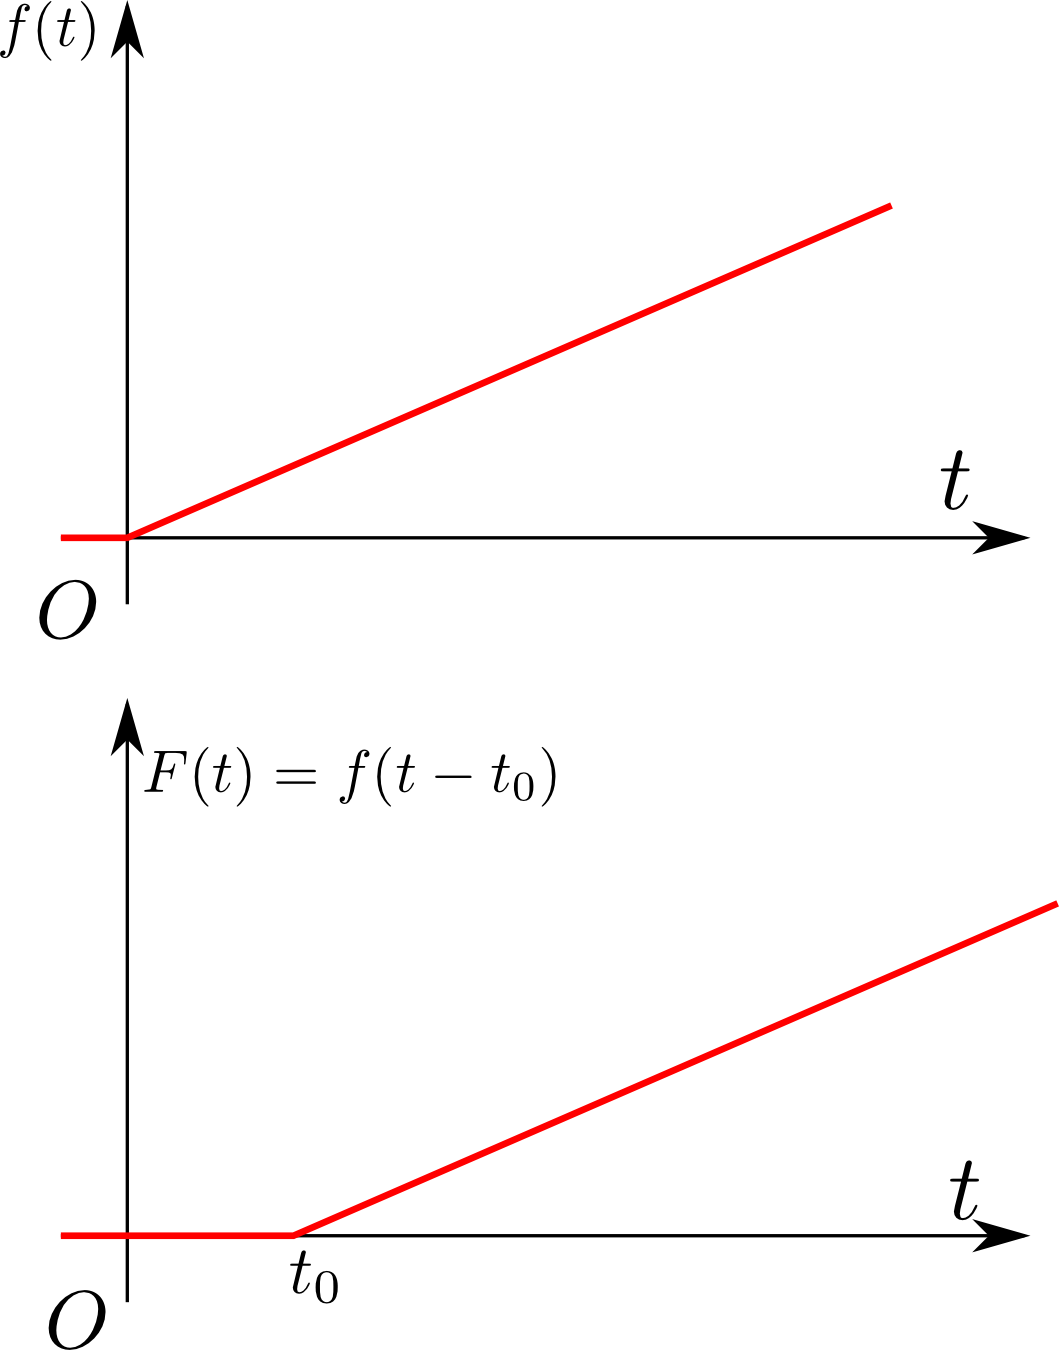
\includegraphics[width=.25\textwidth]{images/retard}
\end{center}
\end{minipage}

Tout retard temporel $t_0$ sur une fonction se traduit par un facteur
multiplicatif $e^{-t_0 p}$ sur sa transformée de Laplace.


\begin{minipage}[c]{.6\linewidth}
\begin{theorem}
\textbf{Théorème de l'amortissement}

\ifthenelse{\boolean{prof}}{%
$$\mathcal{L} \left[ e^{-a t} f\left(t\right) \right] = F(p+a)$$
}{
\rotatebox{90}{
\begin{tabular}{p{2cm}}
\\
\end{tabular}}
}
\end{theorem}
\end{minipage} \hfill
\begin{minipage}[c]{.35\linewidth}
\end{minipage}

\section{Fonctions usuelles}
\subsection{Transformée de Laplace de signaux d'entrée}
\subsubsection*{Réponse impulsionnelle}
Lorsqu'un système est soumis à, son entrée à une impulsion, on parle de réponse impulsionnelle. Il s'agit de générer un signal d'amplitude infinie pendant un temps infinitésimal. 

\begin{minipage}[c]{.6\linewidth}
\begin{defi}
On note l'impulsion de Dirac $\delta(t)$.
$$
\forall t \neq 0 \quad \delta(t)=0.
$$

La transformée de Laplace d'un Dirac est :

\ifthenelse{\boolean{prof}}{%
$$ F(p) =  \mathcal{L} \left[\delta(t)\right] = 1 $$
}{
\rotatebox{90}{
\begin{tabular}{p{2cm}}
\\
\end{tabular}}
}
\end{defi}
\end{minipage} \hfill
\begin{minipage}[c]{.35\linewidth}
\begin{center}
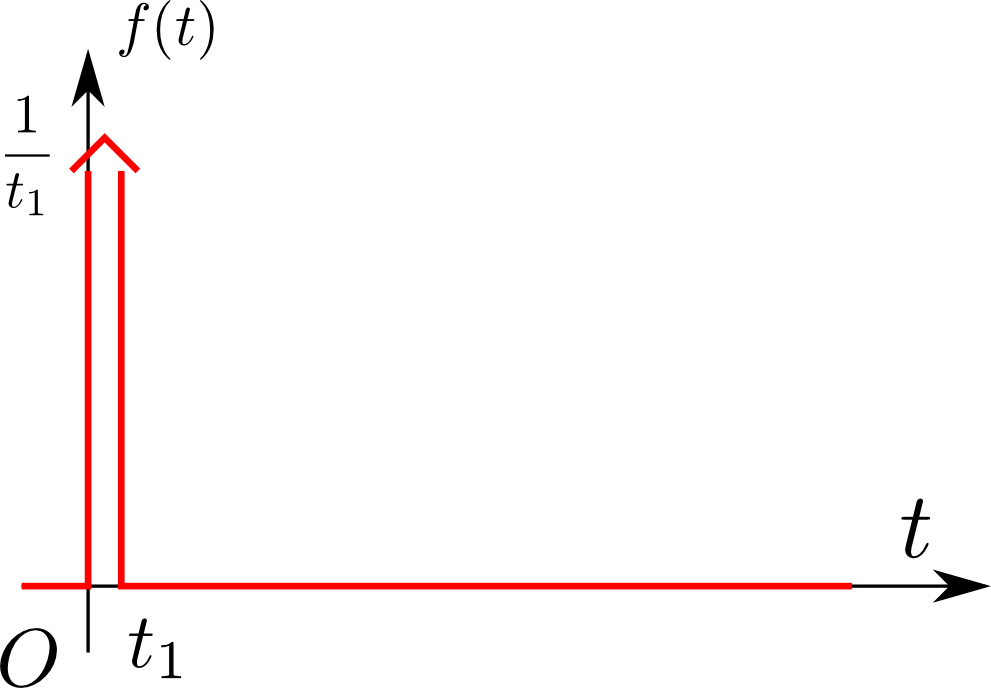
\includegraphics[width=.9\textwidth]{images/dirac}
\end{center}
\end{minipage}


Cette fonction n'a pas de sens physique. Elle permet de modéliser un choc mécanique, un flash ...



\subsubsection*{Réponse indicielle}
\begin{minipage}[c]{.6\linewidth}
\begin{defi}
La réponse indicielle d'un système est la réponse d'un système à une fonction échelon :
$$ \forall t \in \mathbb{R}^+_* \quad f(t)=k \text{ avec } k\in\mathbb{R}$$

La transformée de Laplace d'un échelon d'amplitude $k$ est donnée par :

\ifthenelse{\boolean{prof}}{%
$$F(p) = \mathcal{L} \left[f(t)\right] = \dfrac{k}{p}$$
}{
\rotatebox{90}{
\begin{tabular}{p{2cm}}
\\
\end{tabular}}
}
\end{defi}
\end{minipage} \hfill
\begin{minipage}[c]{.35\linewidth}
\begin{center}
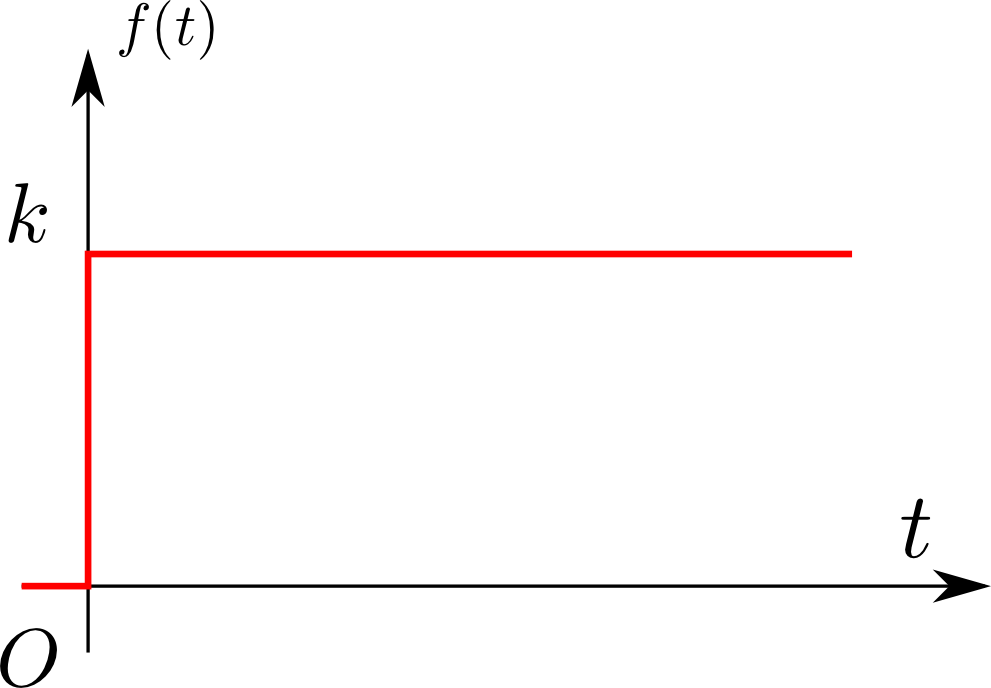
\includegraphics[width=.9\textwidth]{images/echelon}
\end{center}
\end{minipage}





\subsubsection*{Réponse à une rampe et une fonction puissance}
\begin{minipage}[c]{.6\linewidth}
\begin{defi}
Une rampe est une fonction linéaire définie par : 
$$ \forall t \in \mathbb{R}^+_* \quad f(t) = t$$

La transformée de Laplace de $f$ se définit par : 

\ifthenelse{\boolean{prof}}{%
$$ F(p) = \mathcal{L} \left[f(t)\right]  =
\dfrac{1}{p^2} $$
}{
\rotatebox{90}{
\begin{tabular}{p{2cm}}
\\
\end{tabular}}
}
\end{defi}
\begin{defi}
Par extensions, on peut définir les fonctions puissances telles que :
$$ \forall t \in \mathbb{R}^+_* \quad f(t) = t^n$$

La transformée de Laplace est alors :
$$ \forall t\in \mathbb{R}^+_*  \quad
F(p) = \mathcal{L} \left[f(t)\right]  =
\dfrac{n!}{p^{n+1}} $$
\end{defi}
\end{minipage} \hfill
\begin{minipage}[c]{.35\linewidth}
\begin{center}
\includegraphics[width=.9\textwidth]{images/rampe}
\end{center}
\end{minipage}


%\begin{demo}
\textbf{Calcul de $\mathcal{L}\left[f(t) \right]$ avec $f(t)=t\quad \forall t> 0$.}

\ifthenelse{\boolean{prof}}{%
$$
\mathcal{L}\left[f(t) \right] 
= \mathcal{L}\left[t \right] 
= F(p)
= \int\limits_0^{+ \infty} t \cdot e^{-pt}dt
$$

D'après la formule d'intégration par partie : $\int\limits_{a}^{b} u dv  = \left[uv\right]_{a}^{b} - \int\limits_{a}^{b} v du$.

On pose :
\begin{itemize}
\item $u=t$ et donc $\dfrac{du}{dt}=1$ et donc $du=dt$;
\item $dv = e^{-pt}dt$ et donc $v=-\dfrac{1}{p}e^{-pt}$.
\end{itemize}

On a donc :
\begin{eqnarray*}
F(p)
&=& \int\limits_0^{+ \infty} t \cdot e^{-pt}dt
=\left[ - t \dfrac{1}{p}e^{-pt} \right]_{0}^{+\infty} - \int\limits_0^{+ \infty} -\dfrac{1}{p}e^{-pt} dt \\
& =& 0 - \left[\dfrac{1}{p^2} e^{-pt}  \right]_{0}^{+\infty} = \dfrac{1}{p^2}
\end{eqnarray*}

Au final $\mathcal{L}\left[f(t) \right] = \dfrac{1}{p^2}$.

}{
\rotatebox{90}{
\begin{tabular}{p{12cm}}
\\
\end{tabular}}
}
%\end{demo}




\subsection{Transformée de Laplace de fonctions usuelles}
Le calcul de la transformation de Laplace à partir des définitions des fonctions usuelles n'est pas à savoir. En revanche, les transformées les plus courantes doivent être connues. Dans d'autres cas, le tableau des transformées vous sera donnée.
Dans les conditions de Heavisde, on a donc les transformées de Laplace suivantes :

\begin{center}
\begin{tabular}{|c|c||c|c|}
\hline
Domaine temporel $f(t)$ & Domaine de Laplace $F(p)$ & 
Domaine temporel $f(t)$ & Domaine de Laplace $F(p)$ \\
\hline
\hline
 &&& \\
Dirac $\delta(t)$ &
$F(p)=1$ &
Échelon $ u(t)=k $&
$ U(p) = \dfrac{k}{p}$
\\
&&& \\
\hline
&&& \\
Puissances
$f(t) = t^n\cdot u(t)$ &
$F(p)=\dfrac{n!}{p^{n+1}} $ &
Créneau $\forall t\in ]0,t_1 [ \quad f(t)= A$ & 
$F(p) =A \cdot \dfrac{1-e^{-pt_1}}{p} $\\
&&& \\
\hline
&&& \\
$f(t) = \sin \left( \omega_0 t\right) \cdot u(t)$ &
$F(p) = \dfrac{\omega_0}{p^2+\omega_0^2} $ &
$f(t) = \cos \left( \omega_0 t\right) \cdot u(t)$ & 
$F(p) = \dfrac{p}{p^2+\omega_0^2} $ \\
&&& \\
\hline
&&& \\
$f(t)= e^{-at}\cdot u(t)$ & 
$F(p)= \dfrac{1}{p+a}$ &
$f(t) = e^{-at}\sin\left( \omega_0 t\right) \cdot u(t)$ &
$F(p)=\dfrac{\omega_0}{\left( p+a\right)^2 + \omega_0^2}$  \\
&&& \\
\hline
&&& \\
$f(t)$ est $T$ périodique &
$F(p)= \dfrac{\mathcal{L} \left[f_0 (t)\right]}{1-e^{-Tp}} \cdot u(t)$ &
$f(t)=t^ne^{-at}u(t)$ & $F(p)=\dfrac{n!}{\left( p+a\right)^{n+1}}$
\\
&&& \\
\hline
\end{tabular}
\end{center}


%\begin{demo}
\textbf{Calcul de $\mathcal{L}\left[f(t) \right]$ avec $f(t)=e^{-at}\quad \forall t> 0$.}

\ifthenelse{\boolean{prof}}{
$$
\mathcal{L}\left[f(t) \right] 
= \mathcal{L}\left[e^{-at} \right] 
= F(p)
= \int\limits_0^{+ \infty} e^{-at} \cdot e^{-pt}dt
= \int\limits_0^{+ \infty} e^{-\left(p+a\right)t} dt
=\left[
-\dfrac{1}{p+a}e^{-\left(p+a\right)t}
\right]_0^{+ \infty}
=\dfrac{1}{p+a}
$$

Au final $\mathcal{L}\left[f(t) \right] = \dfrac{1}{p+a}$.

}{
\rotatebox{90}{
\begin{tabular}{p{6cm}}
\\
\end{tabular}}
}
%\end{demo}

%\begin{demo}
\textbf{Calcul de $\mathcal{L}\left[f(t) \right]$ avec $f(t)= \sin \left(\omega t \right)\quad \forall t> 0$.}

Calculons :
$$
F(p)= \int\limits_0^{+ \infty} \sin \left(\omega t \right) \cdot e^{-pt}dt
$$

On rappelle que $\int uv'  = [uv]-\int u'v$.

On pose : 
\begin{itemize}
\item $u(t)=\sin \left(\omega t\right)$ et $u'(t)=\omega \cos \left(\omega t\right)$
\item $v'(t)=e^{-pt}$ et $v(t)=-\dfrac{1}{p}e^{-pt}$
\end{itemize}
avec $u$ et $v$ $C^1$ sur $\mathbb{R_+}$.

En conséquence, 
\begin{eqnarray*}
F(p)
&=& \int\limits_0^{+ \infty} \sin \left(\omega t \right) \cdot e^{-pt}dt
= \left[-\dfrac{1}{p}e^{-pt} \cdot \sin \left(\omega t\right) \right]_0^{+ \infty}
- \int\limits_0^{+ \infty} -\dfrac{1}{p}e^{-pt} \omega \cos \left(\omega t\right) dt \\
&=& \left[-\dfrac{1}{p}e^{-pt} \cdot \sin \left(\omega t\right) \right]_0^{+ \infty}
+\dfrac{\omega}{^p}\int\limits_0^{+ \infty} e^{-pt} \cos \left(\omega t\right) dt
\end{eqnarray*}

En réalisant une seconde intégration par partie, on pose $w(t)=\cos \left(\omega t\right)$ et $w'(t)=-\omega \sin \left(\omega t\right)$. On a donc $\int wv'  = [wv]-\int w'v$ :
$$
\int\limits_0^{+ \infty} e^{-pt} \cos \left(\omega t\right) dt
= \left[-\dfrac{1}{p}e^{-pt} \cdot \cos \left(\omega t\right) \right]_0^{+ \infty}
- \dfrac{\omega}{p} \underbrace{\int\limits_0^{+ \infty} e^{-pt} \cdot  \sin \left(\omega t\right) dt}_{F(p)}
$$

En conséquence :

\begin{eqnarray*}
&&F(p)=\left[-\dfrac{1}{p}e^{-pt} \cdot \sin \left(\omega t\right) \right]_0^{+ \infty}
+\dfrac{\omega}{p}\left[-\dfrac{1}{p}e^{-pt} \cdot \cos \left(\omega t\right) \right]_0^{+ \infty}
- \dfrac{\omega}{p}\dfrac{\omega}{p} F(p) \\
&\Longleftrightarrow &
F(p)\left(1+\dfrac{\omega^2}{p^2}\right) =\underbrace{\left[-\dfrac{1}{p}e^{-pt} \cdot \sin \left(\omega t\right) \right]_0^{+ \infty}}_{0}
+\dfrac{\omega}{p}
\underbrace{\left[-\dfrac{1}{p}e^{-pt} \cdot \cos \left(\omega t\right) \right]_0^{+ \infty}}_{\dfrac{1}{p}}\\
&\Longleftrightarrow &
F(p)=\dfrac{\omega}{p^2}\cdot\dfrac{p^2}{p^2+\omega^2} = \dfrac{\omega}{p^2+\omega^2}
\end{eqnarray*}

Au final $\mathcal{L}\left[\sin(\omega t) \right] = \dfrac{\omega}{p^2+\omega^2}$.

%\end{demo}

\section{Transformée de Laplace inverse}

Après avoir trouvé la fonction de transfert du système auquel on ajoute la
fonction de transfert du signal, on se retrouve avec une nouvelle fonction
polynomiale qui est le produit des deux polynômes précédents. 

Pour connaître la fonction globale du système dans le domaine temporel, on doit
effectuer la transformée inverse de Laplace de ce nouveau polynôme. 

La transformation inverse consiste à décomposer la fraction rationnelle (en $p$)
en éléments simples (somme de plusieurs fractions simples en $p$) et à
identifier chaque élément simple à une fonction élémentaire en $t$.

\subsection{Propriétés mathématiques}
Soit $f$ une fonction rationnelle définie par $f(x)
=\dfrac{p(x)}{q(x)}$ où $p$ et $q$ sont deux fonctions polynômes. 

%\begin{prop}
Soit
$$
f(x)=\dfrac{p(x)}{q(x)}=
\dfrac{p(x)}{\left(x-a_1 \right)\left(x-a_2 \right)...\left(x-a_n \right)}
$$
avec $\text{deg}(p)<\text{deg}(q)$ ($a_i\neq a_j,\; \forall (i,j) \in \left\{1,2,3,..n
\right\}^2$ tel que $i\neq j$).

Alors $f(x)$ peut se mettre sous la forme :

$$
f(x)=\dfrac{p(x)}{q(x)}=
\dfrac{\alpha_1}{\left(x-a_1 \right)}
+\dfrac{\alpha_2}{\left(x-a_2 \right)}
+\cdots
+\dfrac{\alpha_n}{\left(x-a_n \right)}
$$

%\end{prop}

\paragraph*{Propriété 2}
%\begin{prop}
Soit
$$
f(x)=\dfrac{p(x)}{q(x)}=
\dfrac{p(x)}{\left(x-a_1 \right)^{p1}\left(x-a_2 \right)^{p2}\cdots\left(x-a_n
\right)^{pn}}
$$
avec $\text{deg}(p)<\text{deg}(q)$ ($a_i\neq a_j,\; \forall (i,j) \in \left\{1,2,3,..n
\right\}^2$ tel que $i\neq j$).

Alors $f(x)$ peut se mettre sous la forme :
$$
\begin{array}{lll}
f(x)=\dfrac{p(x)}{q(x)}&=&
\dfrac{\alpha_{11}}{\left(x-a_1 \right)}
+\dfrac{\alpha_{12}}{\left(x-a_1 \right)^2}
+\cdots
+\dfrac{\alpha_{1p1}}{\left(x-a_1 \right)^{p1}}
+\dfrac{\alpha_{21}}{\left(x-a_2 \right)}
+\dfrac{\alpha_{22}}{\left(x-a_2 \right)^{2}}
+\cdots \\
&&
+\dfrac{\alpha_{2p2}}{\left(x-a_2 \right)^{p2}}
+\dfrac{\alpha_{n1}}{\left(x-a_n \right)}
+\dfrac{\alpha_{n2}}{\left(x-a_n \right)^{2}}
+\cdots
+\dfrac{\alpha_{npn}}{\left(x-a_n \right)^{pn}}
\end{array}
$$

soit : 

$$
f(x)=\sum\limits_{i=1}^n \sum\limits_{j=1}^{pi}
\dfrac{\alpha_{ij}}{\left(x-a_i\right)^j}
$$
%\end{prop}
\paragraph*{Propriété 3}
%\begin{prop}
Soit
$$
f(x)=\dfrac{p(x)}{q(x)}=
\dfrac{p(x)}{
\prod\limits_{i=1}^{n} \left(x-a_i \right)^{p1}
\prod\limits_{k=1}^{m} \left(x^2+b_kx+ck \right)^{qm}
}
$$
avec $\text{deg}(p)<\text{deg}(q)$ ($a_i\neq a_j,\; \forall (i,j) \in \left\{1,2,3,..n
\right\}^2$ tel que $i\neq j$) et $b^2_k-ac_k<0 \; \forall k \in\left\{1,2,..m
\right\}$ 

Alors $f(x)$ peut se mettre sous la forme :
$$
f(x)=\dfrac{p(x)}{q(x)}=
\sum\limits_{i=1}^n \sum\limits_{j=1}^{pi}
\dfrac{\alpha_{ij}}{\left(x-a_i\right)^j}
+
\sum\limits_{k=1}^m \sum\limits_{j=1}^{qk}
\dfrac{\beta_{kj}x}{\left(x^2+b_kx+c_k\right)^j}
$$
%\end{prop}


\end{document}
\subsection{Exemples}
\begin{exemple}
Chercher les transformées inverses des fonctions suivantes : 
\begin{enumerate}%
\item $F(p)=\dfrac{1}{p(p+a)}$
\item $F(p)=\dfrac{3p+7}{p^2-2p-3}$
\item $F(p)=\dfrac{2p^2-4}{\left( p+1\right)
\left( p-2\right)\left( p-3\right)}$
\item $F(p) = \dfrac{p^2+2p+3}{\left( p^2+2p+1\right)\left( p^2+2p+5\right)}$
\end{enumerate}
\end{exemple}


\ifthenelse{\boolean{prof}}{

Déterminer les transformées de Laplace inverse des fonctions suivantes :

$$ F(x)=\dfrac{X+1}{\left(X-1\right)\left(X-2\right)\left(X-3\right)} $$
$$ F(x)=\dfrac{X^2+X+1}{\left(X^2+1\right)\left(X^2-1\right)} $$
$$ F(x)=\dfrac{1}{\left(X+1\right)\left(X^2+X+1\right)^2}$$
$$ F(X)=\dfrac{1}{\left(X^2-1\right)^2}$$

\paragraph*{Pôles simples}
La décomposition de
$F(x)=\dfrac{X+1}{\left(X-1\right)\left(X-2\right)\left(X-3\right)}
$ est de la forme :

$$
F(x)=\dfrac{X+1}{\left(X-1\right)\left(X-2\right)\left(X-3\right)}
=
\dfrac{a}{X-1}
+\dfrac{b}{X-2}
+\dfrac{c}{X-3}
$$

où $a$, $b$ et $c$ sont des constantes puisque $\left(X-1\right)$,
$\left(X-2\right)$ et $\left(X-3\right)$ sont des polynômes premiers entre eux
deux à deux de degré 1.

Pour déterminer $a$ on calcule $\left(X-1\right)F(x)$ en 1 et on trouve $a=1$.

Pour déterminer $b$ on calcule $\left(X-2\right)F(x)$ en 2 et on trouve $b=-3$.

Pour déterminer $c$ on calcule $\left(X-3\right)F(x)$ en 3 et on trouve $c=2$.

La décomposition est alors : 
$$
F(x)=\dfrac{X+1}{\left(X-1\right)\left(X-2\right)\left(X-3\right)}
=
\dfrac{1}{X-1}
-\dfrac{3}{X-2}
+\dfrac{2}{X-3}
$$


\paragraph*{Polynômes irréductibles de R[X] de degré 2}
La fonction $F(x)=\dfrac{X^2+X+1}{\left(X^2+1\right)\left(X^2-1\right)}$ se
décompose sous la forme 
$F(x)=
\dfrac{aX+b}{\left(X^2+1\right)}
+\dfrac{c}{\left(X-1\right)}
+\dfrac{d}{\left(X+1\right)}
$.
Pour déterminer $a$ et $b$, on calcule $\left(X^2+1\right)F(X)$ en $i$,  on
obtient :$\dfrac{-i}{2}=ai+b$. La famille $(1,i)$ étant libre, on en déduit
$a=-\dfrac{1}{2}$ et $b=0$.

% \paragraph*{Utilisation des limites}
% Soit $F(x)=\dfrac{1}{\left(X+1\right)\left(X^2+X+1\right)^2}$. Sa
% décomposition  est de la forme : 
% $$
% F(x)=\dfrac{a}{X+1}
% +\dfrac{}{}
% $$

$F(x)=\dfrac{1}{\left(X+1\right)\left(X^2+X+1\right)^2}$
$F(X)=\dfrac{1}{\left(X^2-1\right)^2}$
\paragraph*{Utilisation de la parité}
Soit $F(X)=\dfrac{1}{\left(X^2-1\right)^2}$. La décomposition est de la forme : 
$$
F(X)=
\dfrac{a}{\left(X-1\right)^2}
+\dfrac{b}{X-1}
+\dfrac{c}{\left(X+1\right)^2}
+\dfrac{d}{X+1}
$$

On a alors :
$$F(-X)=
\dfrac{a}{\left(X+1\right)^2}
+\dfrac{-b}{X+1}
+\dfrac{c}{\left(X-1\right)^2}
+\dfrac{-d}{X-1}
$$

En conséquence $a=c$ et $b=-d$.

En calculant $(X-1)^2F(X)$ en 1 on obtient $a=\dfrac{1}{4}$.
En 0 on trouve $b=\dfrac{-1}{2}$.

\subsection{Exemple}
\begin{exemple}
Chercher les transformées inverses des fonctions suivantes : 
\begin{enumerate}%
\item $F(p)=\dfrac{1}{p(p+a)}$
\item $F(p)=\dfrac{3p+7}{p^2-2p-3}$
\item $F(p)=\dfrac{2p^2-4}{\left( p+1\right)
\left( p-2\right)\left( p-3\right)}$
\item $F(p) = \dfrac{p^2+2p+3}{\left( p^2+2p+1\right)\left( p^2+2p+5\right)}$
\end{enumerate}
\end{exemple}
%\section*{Exercice}
%Chercher les transformées inverses des fonctions suivantes : 
%\begin{enumerate}%
 %\item $F(p)=\dfrac{1}{p(p+a)}$
 %\item $F(p)=\dfrac{3p+7}{p^2-2p-3}$
%\item $F(p)=\dfrac{2p^2-4}{\left( p+1\right)
%\left( p-2\right)\left( p-3\right)}$
%\item $F(p) = \dfrac{p^2+2p+3}{\left( p^2+2p+1\right)\left( p^2+2p+5\right)}$
%\end{enumerate}
}{}
\end{document}
